%%%%%%%%%%%%%%%%%%%%%%%%%%%%%%%%%%%%%%%%%%%%%%%%%%%%%%%%%%%%%%%
%% OXFORD THESIS TEMPLATE


% Use this template to produce a standard thesis that meets the Oxford 
% University requirements for DPhil submission
%
% Originally by Keith A. Gillow (gillow@maths.ox.ac.uk), 1997
% Modified by Sam Evans (sam@samuelevansresearch.org), 2007
% Modified by John McManigle (mcmanigle@gmail.com), 2015

% I've (John) tried to comment this file extensively, so read through it to see 
% how to use the various options.  Remember that in LaTeX, any line starting 
% with a % is NOT executed.  Several places below, you have a choice of which 
% line to use out of multiple options (eg draft vs final, for PDF vs for 
% binding, etc.)  When you pick one, add a % to the beginning of the lines you 
% don't want.


%%%%% CHOOSE PAGE LAYOUT
% The most common choices should be below.  You can also do other things, like 
% replacing "a4paper" with "letterpaper", etc.

% This one will format for two-sided binding (ie left and right pages have 
% mirror margins; blank pages inserted where needed):
%\documentclass[a4paper,twoside]{ociamthesis}

% This one will format for one-sided binding (ie left margin > right margin; no 
% extra blank pages):
%\documentclass[a4paper]{ociamthesis}

% This one will format for PDF output (ie equal margins, no extra blank pages):
\documentclass[a4paper,nobind]{ociamthesis} 



%%%%% SELECT YOUR DRAFT OPTIONS
% Three options going on here; use in any combination.  But remember to turn the 
% first two off before generating a PDF to send to the printer!

% This adds a "DRAFT" footer to every normal page.  (The first page of each 
% chapter is not a "normal" page.)
\fancyfoot[C]{\emph{DRAFT Printed on \today}}  

% This highlights (in blue) corrections marked with (for words) \mccorrect{blah} 
% or (for whole paragraphs) \begin{mccorrection} . . . \end{mccorrection}.  
% This can be useful for sending a PDF of your corrected thesis to your 
% examiners for review.  Turn it off, and the blue disappears.
\correctionstrue


%%%%% BIBLIOGRAPHY SETUP
% Note that your bibliography will require some tweaking depending on your 
% department, preferred format, etc. The options included below are just very 
% basic "sciencey" and "humanitiesey" options to get started. If you've not used 
% LaTeX before, I recommend reading a little about biblatex/biber and getting 
% started with it. If you're already a LaTeX pro and are used to natbib or 
% something, modify as necessary. Either way, you'll have to choose and 
% configure an appropriate bibliography format...

% The science-type option: numerical in-text citation with references in order 
% of appearance.
\usepackage[style=numeric-comp, sorting=none, backend=biber, doi=false, isbn=false]{biblatex}
\usepackage{ amssymb }
\usepackage{slashed}
\newcommand*{\bibtitle}{References}

% This makes the bibliography left-aligned (not 'justified') and slightly 
% smaller font.
\renewcommand*{\bibfont}{\raggedright\small}

% Change this to the name of your .bib file (usually exported from a citation 
% manager like Zotero or EndNote).
\addbibresource{references.bib}


% Uncomment this if you want equation numbers per section (2.3.12), instead of 
% per chapter (2.18):
%\numberwithin{equation}{subsection}


%%%%% THESIS / TITLE PAGE INFORMATION

% Everybody needs to complete the following:
\title{Evaluating the Performance of the ProtoDUNE--SP Detector using Michel Electrons}
\author{Aidan Reynolds}
\college{University College}
\degree{Doctor of Philosophy}
\degreedate{Hilary 2020}

%%%%% YOUR OWN PERSONAL MACROS

% This is a good place to dump your own LaTeX macros as they come up.
\newcommand{\fig}[1]{Fig. \ref{#1}}

% To make text superscripts shortcuts
\renewcommand{\th}{\textsuperscript{th}} 
\newcommand{\nd}{\textsuperscript{nd}}
\renewcommand{\st}{\textsuperscript{st}}
\newcommand{\rd}{\textsuperscript{rd}}


%%%%% THE ACTUAL DOCUMENT STARTS HERE
\begin{document}

%%%%% CHOOSE YOUR LINE SPACING HERE

% This is the official option.  Use it for your submission copy and library copy:
\setlength{\textbaselineskip}{22pt plus2pt}

% This is closer spacing (about 1.5-spaced) that you might prefer for your 
% personal copies:
%\setlength{\textbaselineskip}{18pt plus2pt minus1pt}

% You can set the spacing here for the roman-numbered pages (acknowledgements, 
% table of contents, etc.)
\setlength{\frontmatterbaselineskip}{17pt plus1pt minus1pt}

% Leave this line alone; it gets things started for the real document.
\setlength{\baselineskip}{\textbaselineskip}


%%%%% CHOOSE YOUR SECTION NUMBERING DEPTH HERE
% You have two choices.  First, how far down are sections numbered?  (Below 
% that, they're named but don't get numbers.)  Second, what level of section 
% appears in the table of contents?  These don't have to match: you can have 
% numbered sections that don't show up in the ToC, or unnumbered sections that
% do.  Throughout, 0 = chapter; 1 = section; 2 = subsection; 3 = subsubsection, 
% 4 = paragraph...

% The level that gets a number:
\setcounter{secnumdepth}{3}
% The level that shows up in the ToC:
\setcounter{tocdepth}{3}


%%%%% ABSTRACT SEPARATE
% This is used to create the separate, one-page abstract that you are required 
% to hand into the Exam Schools. You can comment it out to generate a PDF for 
% printing or whatnot.
% \begin{abstractseparate}
% 	This thesis presents the results of a study of electromagnetic interactions in 
the \protodune{} liquid argon time projection chamber (LArTPC) detector. The 
LArTPC detector technology provides high spatial resolution on the final states 
of neutrino interactions, allowing interaction modes to be distinguished based 
on the geometry of the interactions in the event. In order to perform high
precision measurements of neutrinos in LArTPC detectors, final state particles
need to be effectively identified, and their energy accurately reconstructed.
This work focussed on these challenges with two studies on data from the
\protodune{} LArTPC, a study of track--shower classification, and a study of 
Michel electron energy reconstruction. A track--shower classification algorithm
is developed based on the use of convolutional neural networks, and its
performance is compared to the current track--shower classification algorithm.
Michel electrons are used as a source of electromagnetic activity in the tens of
MeV range, and the energy resolution and bias for these electrons are estimated.

% In
% this work, track--shower discrimination and Michel electron reconstruction are 
% studied in the \protodune{} LArTPC. 
% 
% A track--shower discriminator based on
% convolutional neural networks was developed, and shows a 
% 
% A convolutional neural network is trained 
% for track--shower classification, 
% 
%     which demonstrates a significant improvement
% over the current algorithms in terms of 
% 
% 
% In order to perform high 
% precision measurements of supernova neutrinos in LArTPC detectors, electrons 
% must be identified and their energy accurately reconstructed. In this work EM 
% activity is studied in the 10--50 MeV range using Michel electrons as a source 
% with a well defined energy spectrum. The energy uncertainty and bias for
% reconstructed Michel electron events in the \protodune{} LArTPC are estimated.
% 
% The sensitivity, bias, and energy scale are 
% studied and the implications for neutrino physics in the Deep Underground 
% Neutrino Experiment are discussed.
 
% \end{abstractseparate}


% JEM: Pages are roman numbered from here, though page numbers are invisible 
% until ToC.  This is in keeping with most typesetting conventions.
\begin{romanpages}

% Title page is created here
\maketitle

%%%%% DEDICATION -- If you'd like one, un-comment the following.
%\begin{dedication}
%This thesis is dedicated to\\
%someone\\
%for some special reason\\
%\end{dedication}

%%%%% ACKNOWLEDGEMENTS -- Nothing to do here except comment out if you don't want it.
% \begin{acknowledgements}
% 	This thesis would not have been possible without the advice and support of many
people. I would like to start by thanking my supervisor, Alfons Weber. He has
been a brilliant advisor, and I would like to thank him in particular for all
the opportunities he has given me. Thanks also to the rest of the Oxford
Neutrino Physics group, particularly Justo Martin--Albo whose support during 
my first year helped me to settle into the DPhil, and my fellow students -- 
Fabio, Alex, and Ciaran -- who have made the office, both physical and 
virtual, an enjoyable place to work.

\bigskip\noindent
I have worked with many great collaborators from the DUNE experiment
as part of my DPhil. I'd particularly like to thank the members of the 
\protodune{} reconstruction and analysis group who have always given 
excellent feedback on my work. Special thanks go to Dorota Stefan and Robert 
Sulej, who were incredibly supportive during the early years of my DPhil, and 
to Leigh Whitehead and Tingjun Yang, whose insightful conversations have been 
invaluable. 

\bigskip\noindent
I am very fortunate to have had the chance to work at CERN for part of my DPhil,
and I would like to thank all of the members of the on--site \protodune{} 
team. Especially Alex, Chris, Geoff, James, Milo, and Seb, who I thoroughly 
enjoyed working with during my time at CERN, and who I have learned so much 
from. 

\bigskip\noindent
Finally, my greatest thanks go to my friends and family, for their continued
support over the years. To Amy, Rory, and Helena, who have always been there to
help me relax at the end of the day; to the members of Oxford Ultimate, who have
been so welcoming over the past year, you have kept me going during the final 
stages; to my family, who fostered a love of learning, which will always be 
with me; and to Ellie, who could never understand how much her support has 
meant to me over the years.

% \end{acknowledgements}

%%%%% ABSTRACT -- Nothing to do here except comment out if you don't want it.
\begin{abstract}
	This thesis presents the results of a study of electromagnetic interactions in 
the \protodune{} liquid argon time projection chamber (LArTPC) detector. The 
LArTPC detector technology provides high spatial resolution on the final states 
of neutrino interactions, allowing interaction modes to be distinguished based 
on the geometry of the interactions in the event. In order to perform high
precision measurements of neutrinos in LArTPC detectors, final state particles
need to be effectively identified, and their energy accurately reconstructed.
This work focussed on these challenges with two studies on data from the
\protodune{} LArTPC, a study of track--shower classification, and a study of 
Michel electron energy reconstruction. A track--shower classification algorithm
is developed based on the use of convolutional neural networks, and its
performance is compared to the current track--shower classification algorithm.
Michel electrons are used as a source of electromagnetic activity in the tens of
MeV range, and the energy resolution and bias for these electrons are estimated.

% In
% this work, track--shower discrimination and Michel electron reconstruction are 
% studied in the \protodune{} LArTPC. 
% 
% A track--shower discriminator based on
% convolutional neural networks was developed, and shows a 
% 
% A convolutional neural network is trained 
% for track--shower classification, 
% 
%     which demonstrates a significant improvement
% over the current algorithms in terms of 
% 
% 
% In order to perform high 
% precision measurements of supernova neutrinos in LArTPC detectors, electrons 
% must be identified and their energy accurately reconstructed. In this work EM 
% activity is studied in the 10--50 MeV range using Michel electrons as a source 
% with a well defined energy spectrum. The energy uncertainty and bias for
% reconstructed Michel electron events in the \protodune{} LArTPC are estimated.
% 
% The sensitivity, bias, and energy scale are 
% studied and the implications for neutrino physics in the Deep Underground 
% Neutrino Experiment are discussed.

\end{abstract}

%%%%% MINI TABLES
% This lays the groundwork for per-chapter, mini tables of contents.  Comment 
% the following line (and remove \minitoc from the chapter files) if you don't 
% want this.  Un-comment either of the next two lines if you want a per-chapter 
% list of figures or tables.
\dominitoc % include a mini table of contents
%\dominilof  % include a mini list of figures
%\dominilot  % include a mini list of tables

% This aligns the bottom of the text of each page.  It generally makes things 
% look better.
\flushbottom

% This is where the whole-document ToC appears:
% TODO: put me back in
\tableofcontents

% TODO: put me back in
\listoffigures
\mtcaddchapter
% \mtcaddchapter is needed when adding a non-chapter (but chapter-like) entity 
% to avoid confusing minitoc

% Uncomment to generate a list of tables:
%\listoftables
%	\mtcaddchapter

%%%%% LIST OF ABBREVIATIONS
% This example includes a list of abbreviations.  Look at text/abbreviations.tex 
% to see how that file is formatted. The template can handle any kind of list 
% though, so this might be a good place for a glossary, etc.

% TODO: put me back in
\begin{mclistof}{List of Abbreviations}{3.2cm}
	\item [ Adam       ] {Adaptive Momentum Estimation}
	\item [ ANN        ] {Artificial Neural Network}
	\item [ APA        ] {Anode--plane Assembly}
	\item [ BI         ] {Beam Instrumentation}
	\item [ CC         ] {Charged Current}
	\item [ CE         ] {Cold Electronics}
	\item [ CNN        ] {Convolutional Neural Network}
	\item [ CP         ] {Charge--Parity}
	\item [ CPT        ] {Charge--Parity--Time}
	\item [ CPA        ] {Cathode--plane Assembly}
	\item [ CRT        ] {Cosmic--ray Tagger}
	\item [ CTB        ] {Central Trigger Board}
	\item [ DAQ        ] {Data Acquisition System}
	\item [ DIS        ] {Deep Inelastic Scattering}
	\item [ DUNE       ] {Deep Underground Neutrino Experiment}
	\item [ ES         ] {Elastic Scattering}
	\item [ FELIX      ] {Front--end Link Exchange}
	\item [ FEMB       ] {Front--end Mother Board}
	\item [ FFT        ] {Fast Fourier Transform}
	\item [ FNAL       ] {Fermilab National Accelerator Laboratory}
	\item [ IO         ] {Inverted Ordering}
	\item [ KamLAND    ] {Kamioka Liquid Scintillator Anti--neutrino Detector}
	\item [ LArTPC     ] {Liquid Argon Time Projection Chamber}
	\item [ LEP        ] {Large Electron--Positron Collider}
	\item [ LHC        ] {Large Hadron Collider}
	\item [ LIGO       ] {Laser Interferometer Gravitational--Wave Observatory}
	\item [ LNGS       ] {Laboratori Nazionali del Gran Sasso}
	\item [ MC         ] {Monte--carlo Simulation}
	\item [ MIP        ] {Minimum Ionising Particle}
	\item [ ML         ] {Machine Learning}
	\item [ MLP        ] {Multi--layer Perceptron}
	\item [ MSW        ] {Mikheyev--Smirnov--Wolfenstein}
	\item [ NC         ] {Neutral Current}
	\item [ NN         ] {Neural Network}
	\item [ NO         ] {Normal Ordering}
	\item [ OM         ] {Online Monitoring}
	\item [ PDS        ] {Photon Detection System}
	\item [ PFParticle ] {Paricle Flow Particle}
	\item [ PID        ] {Particle Identification}
	\item [ PMNS       ] {Pontecorvo--Maki--Nakagawa--Sakata}
	\item [ QE         ] {Quasi--elastic}
	\item [ RCE        ] {Reconfigurable Computing Element}
	\item [ ReLU       ] {Rectified Linear Unit}
	\item [ RES        ] {Resonance}
	\item [ ResNet     ] {Residual Neural Network}
	\item [ RMS        ] {Root Mean Square Deviation}
	\item [ ROC        ] {Reciever Operator Characteristic}
	\item [ SCE        ] {Space Charge Effect}
	\item [ SGD        ] {Stochastic Gradient Descent}
	\item [ SiPM       ] {Silicon Photo--multiplier}
	\item [ SM         ] {Standard Model}
	\item [ SNO        ] {Sudbury Neutrino Observatory}
	\item [ SP         ] {Single Phase}
	\item [ SSM        ] {Standard Solar Model}
	\item [ SSP        ] {SiPM Signal Processor}
	\item [ SURF       ] {Sanford Underground Research Facility}
	\item [ TOF        ] {Time of Flight}
	\item [ TPB        ] {Tetraphenyl-butadiene}
	\item [ TSE        ] {Track--Shower--Empty}
	\item [ WIB        ] {Warm Interface Board}
\end{mclistof} 


% The Roman pages, like the Roman Empire, must come to its inevitable close.
\end{romanpages}


%%%%% CHAPTERS
% Add or remove any chapters you'd like here, by file name (excluding '.tex'):
\flushbottom
\chapter{\label{ch:1-intro}Introduction} 

% \minitoc

Since the discovery of neutrino flavour oscillations, which implies that
neutrinos have mass, neutrino physics has enjoyed a period of rapid development.
The field has begun to transition into an era of precision, with many of the
parameters governing these oscillations having been well constrained. The fact
that neutrinos have mass, and the success of the PMNS theory in describing
neutrino oscillations, leads to a number of fundamental questions which have
important implications in both particle physics and cosmology: 

\begin{itemize}
	\item What is the mechanism giving rise to neutrino mass? 
	\item Are neutrinos Dirac or Majorana particles?
	\item What is the absolute scale and ordering of the neutrino masses?
	\item Do neutrinos and anti--neutrinos oscillate differently, and would this 
	      help to explain the matter anti--matter asymmetry in the universe?
\end{itemize}

In addition to these questions from the neutrino physics community, the high
resolution and large masses of modern neutrino detectors make them useful tools
for both astronomy and astrophysics. 2017 has widely been considered as the dawn
of multi--messenger astronomy, with a measurement of gravitational waves at LIGO
being correlated with measurements of a neutron star merger from electromagnetic
telescopes \cite{Abbott2017}. This measurement was shortly followed by a similar
correlation but in the neutrino sector between a high energy neutrino event in
ICECUBE and a number of traditional telescopes \cite{Aartsen2018}. Within our
galaxy, neutrino detectors provide a unique opportunity to understand the
underlying mechanisms in supernovae; in the case of such a supernova, the
structure of the neutrino flux at earth provides a mechanism to measure effects
in the early stages of the supernova burst which are inaccessible with
electromagnetic measurements \cite{Scholberg:2012id}.

Each of these questions places unique constraints on the design of an
appropriate neutrino detector. The discovery of a matter anti--matter asymmetry
in neutrino oscillations can be answered by making precise measurements of
neutrino oscillations. This requires reliably identifying the flavour and energy
of neutrinos in order to measure the appearance and disappearance spectra
associated with neutrinos produced in long baseline neutrino experiments. To
identify the low energy electrons produced in supernova neutrino interactions, a
detector with low thresholds and low backgrounds is required. The Deep
Underground Neutrino Experiment (DUNE) aims to tackle these challenges by
utilising the Liquid Argon Time Projection Chamber (LArTPC) technology, whose
high spatial and calorimetric resolution allows for more accurate topological
classification of neutrino interactions \cite{Acciarri:2016crz}. To achieve
these goals, a significant programme of LArTPC research is ongoing with
construction, reconstruction, and analysis methods all under development in a
number of LArTPC based experiments \cite{Acciarri:2016smi, Cavanna:2014iqa,
Antonello:2015lea, Abi:2017aow}. 

This thesis presents an analysis of charged particle interactions in the
ProtoDUNE--SP LArTPC detector. A hit classification algorithm is developed and a
sample of Michel electrons is used to provide a measurement of electron energy
bias for low energy electrons. The analysis described in this thesis uses data
collected with the ProtoDUNE--SP detector between August and November 2018.

Michel electrons have an energy spectrum spanning 0--60 MeV; understanding
electrons in this energy range is important as they are the same energy as those
produced when neutrinos from supernova bursts interact. In a LArTPC at these
energies, the energy deposition of electrons transitions between ionisation
dominated and radiation dominated regimes making for a particularly complicated
combined event topology \cite{Acciarri:2017sjy}. The work presented here details
a reconstruction strategy based on augmenting hit identification from a
convolution neural network with simple clustering to identify and reconstruct
Michel electron events. Analysis of these Michel electron events in
ProtoDUNE--SP data and simulation quantifies the energy scale and energy scale
bias for low energy electrons in a surface level LArTPC detector; this
measurement can provide valuable input to studies of supernova burst neutrinos
in LArTPC detectors.

Chapter \ref{ch:2-neutrinophysics} provides a theoretical overview of neutrinos
within the standard model. Interactions, oscillations, and production will be
discussed summarising the current knowledge in the field, as well as open
questions which will be studied in ongoing and upcoming experiments. The role of
neutrinos in supernova bursts and the detection of such neutrinos in a LArTPC
detector will be discussed in more detail.

The ProtoDUNE--SP experiment is described in chapter \ref{ch:3-protodune},
including details of the beam line, detector, cosmic ray flux, and simulations.
An overview of the LArTPC detection principle will be given with specific
details of the ProtoDUNE--SP design. Some details of detector operations will be
discussed, paying particular attention to the monitoring of the detector via the
online data quality monitoring system.

Chapter \ref{ch:4-energyloss} will cover details of electromagnetic energy loss
in liquid argon. Electron and photon energy loss will be discussed as well as
processes leading to electron-ion recombination. The impacts of these effects on
electron reconstruction in liquid argon will be highlighted.

The main analysis of this thesis will be described in chapters
\ref{ch:5-chargeid} and \ref{ch:6-michel}. Details of a hit classification
algorithm based on convolutional neural networks will be given and Michel
electron reconstruction will be highlighted as an example use for the output of
this algorithm. Michel electron production and energy loss in liquid argon will
be discussed. This will be followed by details of the reconstruction strategy
used in the Michel electron analysis. The reconstructed Michel electron spectrum
will be compared between data and simulation, and the energy resolution and
energy scale bias for low energy electrons in the ProtoDUNE--SP detector will be
estimated. 

Chapter \ref{ch:7-implications} will analyse the implications of the results of
the Michel electron analysis for supernova neutrino physics in the DUNE
experiment; the impacts of energy scale bias on these analyses will be
investigated, and the possible performance of DUNE assuming the measured bias
will be discussed.

A summary of the results presented in this thesis will be given in chapter
\ref{ch:8-conclusions} along with a discussion of the implications of these
results for neutrino physics in LArTPC detectors.

\chapter{\label{ch:2-neutrinophysics}Neutrino Physics} 

%%%%%%%%%%%%%%%%%%%%%%%%%%%%%%%%%%%%%%%%%%%%%%%%%%%%%%%%%%%%%%%%%%%%%%%%%%%%%%%%
% From my COS report

% This chapter will cover details of relevant neutrino physics for the thesis 
% project. The theoretical aspects of neutrino physics will be reviewed 
% including the theory of neutrino oscillations in the PMNS framework. 
% Neutrino production will also be discussed including details of neutrino 
% production in supernovae and the role neutrinos can have in understanding 
% the mechanics of a supernova burst
 
% The work for this section is ongoing as it is associated with the analysis 
% work in the other sections, it is expected to be completed by the end of 
% December 2019.
%%%%%%%%%%%%%%%%%%%%%%%%%%%%%%%%%%%%%%%%%%%%%%%%%%%%%%%%%%%%%%%%%%%%%%%%%%%%%%%%

% TODO TODO TODO TODO TODO TODO TODO TODO TODO TODO TODO TODO TODO
% References
% Decide on historical vs theoretical overview or both
% TODO TODO TODO TODO TODO TODO TODO TODO TODO TODO TODO TODO TODO

% \minitoc

Despite being one of the most abundant particle in the universe, neutrinos are 
some of the most elusive; due to the fact that neutrinos can only interact via
the weak interaction. The history of neutrino physics is therefore strongly
connected to the discovery and study of weak interactions. Measurements by
Chadwick in 1914 showed that the energy spectrum of electrons released in
\(\beta\)--decays was continuous, this is in contrast to discrete spectra
observed in \(\alpha\) and \(\gamma\) decays, and seemingly violates
conservation of energy under the assumption of a two--body final state which was
expected at the time. In order to solve this problem, Pauli postulated that the
continuous energy spectrum could be explained if the energy released in a 
\(\beta\)--decay could be shared with an additional neutral weakly interacting 
fermion which Pauli named the neutron. Fermi later renamed Pauli's fermion to
the neutrino, after Chadwick discovered the neutron in 1932. Despite claims that
neutrinos might never be detected, neutrinos have now been discovered and they
have been found to have a number of interesting properties which were not
anticipated when neutrinos were first postulated. This chapter will detail some 
of the history and theory of neutrino's and their interactions.

In this chapter, Section \ref{nu_hist} will give a brief historical overview of 
neutrino physics, Section \ref{nu_osc} will introduce neutrino oscillations
and the theory used to describe them, while Section \ref{nu_prod} will discuss
neutrino interactions in matter as well as neutrino production. Finally Section
\ref{nu_sn} will discuss the production of neutrinos in supernovae, as well as
the role they could play in understanding supernovae.

\section{A Brief History of Neutrino Physics} \label{nu_hist}

The first attempt to incorporate the neutrino into a theoretical model came in
1934 when Fermi presented his theory of \(\beta\)--decay, in this theory the 
neutrino takes part in a four--point interaction with the other components of 
the \(\beta\)--decay interaction. The incredible success of this theory in
explaining the observed properties of \(\beta\)--decays provided strong evidence 
for the neutrinos existence, however, in 1934 after using Fermi's  theory to 
predict the strength of neutrino interactions, H. Bethe and R. Peierls found 
that the interactions were so weak that they might never be observed, a 
prediction that held true for over 20 years.

The first breakthrough in experimental neutrino physics would come in 1956. F.
Reines and C. Cowan were attempting to measure positrons produced in inverse 
\(\beta\)--decay interactions,
\begin{equation}
	\bar{\nu_e} + p \rightarrow n + e^+.
\end{equation}
A detector containing 1400 litres of liquid scintillator was used to measure the 
large flux of electron anti--neutrinos in the vicinity of the Savannah River 
nuclear reactor. They observed a large increase in the rate of positron events 
when the reactor was on when compared to when the reactor was switched off, the 
first experimental evidence for the existence of neutrinos. 

The discovery of the electron neutrino opened the door to answer questions of 
neutrino flavour. As neutrinos are produced alongside a charged lepton it is 
natural to compare the properties of neutrinos with their partners in the weak
interaction. At the time of the discovery of the neutrino there were two known
charged leptons, the electron and the muon, and so physicists asked whether the
neutrinos produced alongside muons are different from those produced alongside
electrons. In 1962, Lederman et al discovered the muon neutrino at Brookhaven
National Laboratory; by creating a beam of muon associated neutrinos using 
decaying pions, and observing the leptons produced in neutrino interactions 
after all other particles had been absorbed. They found that only muons where 
produced in the resulting neutrino interactions, and therefore the neutrinos 
produced were only ever associated with a muon, which shows that neutrinos are 
produced with a distinct flavour in weak interactions.

With the discovery of the tau--lepton in 1977 it was expected that there should 
be an associated tau neutrino, however, it wouldn't be detected until 2001 by 
the DONUT experiment. In the experiment, tau neutrinos where produced from the
decay of charmed mesons produced in collisions between protons and a stationary
target. The neutrino interactions where detected in emulsion detectors, where
the unique geometry of the interaction, in which a short tau track is produced
at the vertex followed by a long muon track, allowed them to be distinguished 
from other decays.

While additional neutrino species are possible, data from measurements of the Z 
boson line--shape at LEP in 1992 restricts the number of active light neutrino 
species to be three. An active light neutrino is any neutrino with \(m_\nu <
\frac{m_Z}{2}\) that can interact with the Z boson, such that the decay \(Z 
\rightarrow \nu \nu \) is possible.

Alongside the discovery of three different types of neutrino, there were
interesting results when observing neutrinos produced in the Sun. The flux of
neutrinos from the Sun at the earth surface had been predicted with Bachall's 
Standard Solar Mode, however, in 1968 when Davis et al measured the flux in the
Homestake experiment they found a deficit with respect to the prediction of the
model, the so called solar neutrino problem. In the Homestake experiment
electron neutrinos where being measured via there inverse beta decay 
interactions with the chlorine in the target,
\begin{equation}
	v_e + ^{37}\mbox{Cl} \rightarrow ^{37}\mbox{Ar} + e^-.
\end{equation}
The neutrino interaction rate was measured by counting the number of argon 
atoms in the chlorine tank by capturing them on helium gas which was
periodically bubbled through the chamber.

In addition to the solar neutrino problem, a similar deficit was observed in
1988 for muon neutrinos produced during cosmic ray showers in the atmosphere.
The Kamiokande experiment was able to measure both electron and muon neutrino 
interactions via the cerenkov radiation produced by the charged leptons in 
water, their data was consistent with the expected rate of electron neutrinos 
from the atmosphere, however, a deficit of muon neutrinos was observed. 

The next generation of the Kamiokande experiment, Super Kamiokande, aimed to
understand the observed deficit of atmospheric muon neutrinos with a larger 
water cerenkov detector capable of resolving the angular distribution of 
atmospheric neutrino interactions. Super Kamiokande consists of a cylindrical 
vessel containing 50kt of ultra pure water, surrounded by an array of around 13
,000 photomultiplier tubes to detect the cerenkov light. Electron and muon 
neutrinos can be distinguished based on the pattern of cerenkov light that is 
left in the detector; due to their higher mass muons leave clear cerenkov 
rings in the detector while electrons, which can scatter and shower, tend to 
leave diffuse "fuzzy" rings on the wall of the detector. In 1998, Super 
Kamiokande published measurements of the flux of atmospheric muon neutrinos as 
a function of azimuthal angle. Since these neutrinos are created a short 
distance from the earths surface, the incoming angle of the neutrino can be 
used to estimate the distance travelled by the neutrino before arriving at the 
detector; the down--going neutrinos have only travelled a short distance in 
the atmosphere (\(\sim 10\mbox{km}\)), while the up--going neutrinos have 
travelled through the entire earth to reach the detector (\(\sim 13,000\mbox{km
}\)). Figure \ref{fig:sk_flux}, shows the flux of neutrinos measured by Super 
Kamiokande as a function of distance travelled; the muon neutrino flux is 
consistent with the no oscillation prediction at small \(\mbox{L} / \mbox{E}_\
nu\), however, for large \(\mbox{L} / \mbox{E}_\nu\) a clear deficit is 
observed. 

\begin{figure}
	\centering
	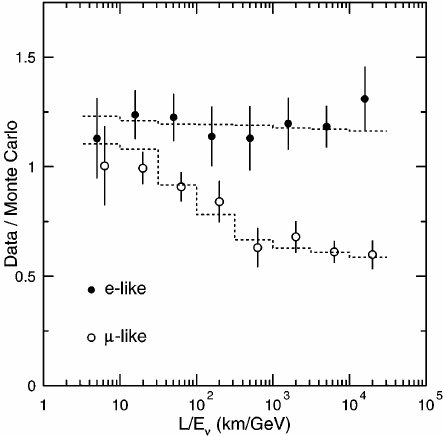
\includegraphics[width=0.7\textwidth]{figures/sk_flux.jpg}
	\caption{Ratio of data to Monte Carlo for electron and muon neutrino fluxes 
	measured by the Super Kamiokande experiment as a function of 
	\(\mbox{L} / \mbox{E}_\nu\). The Monte Carlo prediction is based on the
	assumption of no oscillations. The muon neutrino flux is consistent with the
	no oscillation prediction at small \(\mbox{L} / \mbox{E}_\nu\), however, for
	large \(\mbox{L} / \mbox{E}_\nu\) a clear deficit is observed. The best fit
	under the assumption of atmospheric (\(\nu_\mu \rightarrow \nu_\tau\))
	oscillations is shown, the best fit parameters are \(\Delta m^2 = 2.2 \times
	10^{-3} \mbox{eV}^2\), and \(sin^22\theta = 1\). TODO: ref}
	\label{fig:sk_flux}
\end{figure}

While it wouldn't completely solve the solar neutrino problem, the Sudbury
Neutrino Observatory (SNO) was able to provide unique insight into the observed
solar neutrino fluxes in 2002. Unlike other water cerenkov detectors, SNO 
was filled with heavy water, \(\mbox{D}_2\mbox{O}\), instead of its lighter 
isotope. The use of heavy water in the detector gives rise to additional 
neutrino interactions which allowed the SNO experiment to distinguish between 
three different interaction modes: charged current (CC), neutral current (NC), 
and elastic scattering (ES). Each interaction mode is sensitive to different 
parts of the solar neutrino flux, including some sensitivity to the muon 
neutrino and tau neutrino fluxes.  

%%%%%%%%%%%%%%%%%%%%%%%%%%%%%%%%%%%%%%%%%%%%%%%%%%%%%%%%%%%%%%%%%%%%%%%%%%%%%%%%
% TODO
% Neutral Current & gargamelle??????
% SK
% SNO
% Kamland
% Opera
% precision with daya bay etc.
%%%%%%%%%%%%%%%%%%%%%%%%%%%%%%%%%%%%%%%%%%%%%%%%%%%%%%%%%%%%%%%%%%%%%%%%%%%%%%%%

% \section{Neutrinos in the Standard Model} \label{nu_sm}

\section{Neutrino Oscillations} \label{nu_osc}

\section{Neutrino Interactions} \label{nu_prod}

\section{Supernova Neutrinos} \label{nu_sn}

\chapter{\label{ch:3-protodune}The ProtoDUNE--SP Experiment} 

\minitoc

%%%%%%%%%%%%%%%%%%%%%%%%%%%%%%%%%%%%%%%%%%%%%%%%%%%%%%%%%%%%%%%%%%%%%%%%%%%%%%%%
% From COS
%
% This chapter will discuss the ProtoDUNE--SP experiment and it's role in the
% development of the proposed DUNE experiment. The LArTPC technology will be
% detailed in the general case and then the specifics of the ProtoDUNE--SP
% detector will be given. Details of the major particle fluxes in ProtoDUNE--SP
% will be outlined, along with a discussion of the simulation and reconstruction
% of each flux. Finally, as my main contribution to detector operations during
% data taking was developing for the ProtoDUNE--SP online monitoring system, this
% will be discussed in more depth. 
% 
% The work for the online monitoring subsection has been completed as part of my
% duties as an on--site expert at CERN. I expect to be able to complete the rest
% of the work by the end of December 2019 alongside the other analysis work.
%%%%%%%%%%%%%%%%%%%%%%%%%%%%%%%%%%%%%%%%%%%%%%%%%%%%%%%%%%%%%%%%%%%%%%%%%%%%%%%%

% TODO: image of experiment? 
\protodune{} is one of two prototypes for the DUNE far detector modules that has
been operating at the Neutrino Platform at CERN since the summer of 2018. The
experiment collected data from a charged particle beam for approximately 3 
months before Long Shutdown 2 of the Large Hadron Collider. Since then a 
programme of cosmic ray data collection has been ongoing.

% TODO: Chapter outline
This chapter will outline the technical details of the \protodune{} experiment.
Section \ref{sec:pdsp_dune} will outline the role of \protodune{} in the context
of the DUNE experiment. This will be followed by a discussion of the main
elements of the experiment, the \protodune{} detector systems and the H4
beam line, in Sections \ref{sec:pdsp_detector} and \ref{sec:h4} respectively.
The high event rate in \protodune{} is dominated by a high flux of cosmic rays
which will be discussed in Section \ref{sec:pdsp_cosmic}. Section
\ref{sec:pdsp_sim_reco} will then discuss the simulation and reconstruction of 
\protodune{} data. Finally Section \ref{sec:pdsp_om} will cover details of the 
online monitoring system in \protodune{}; as the primary developer and expert 
on the \protodune{} online monitoring system during my time at CERN, the 
development and maintenance of this system represent a significant body of 
work over 12 months.  

\section{The DUNE Experiment and \protodune{}} \label{sec:pdsp_dune}

\begin{figure}

	\centering

	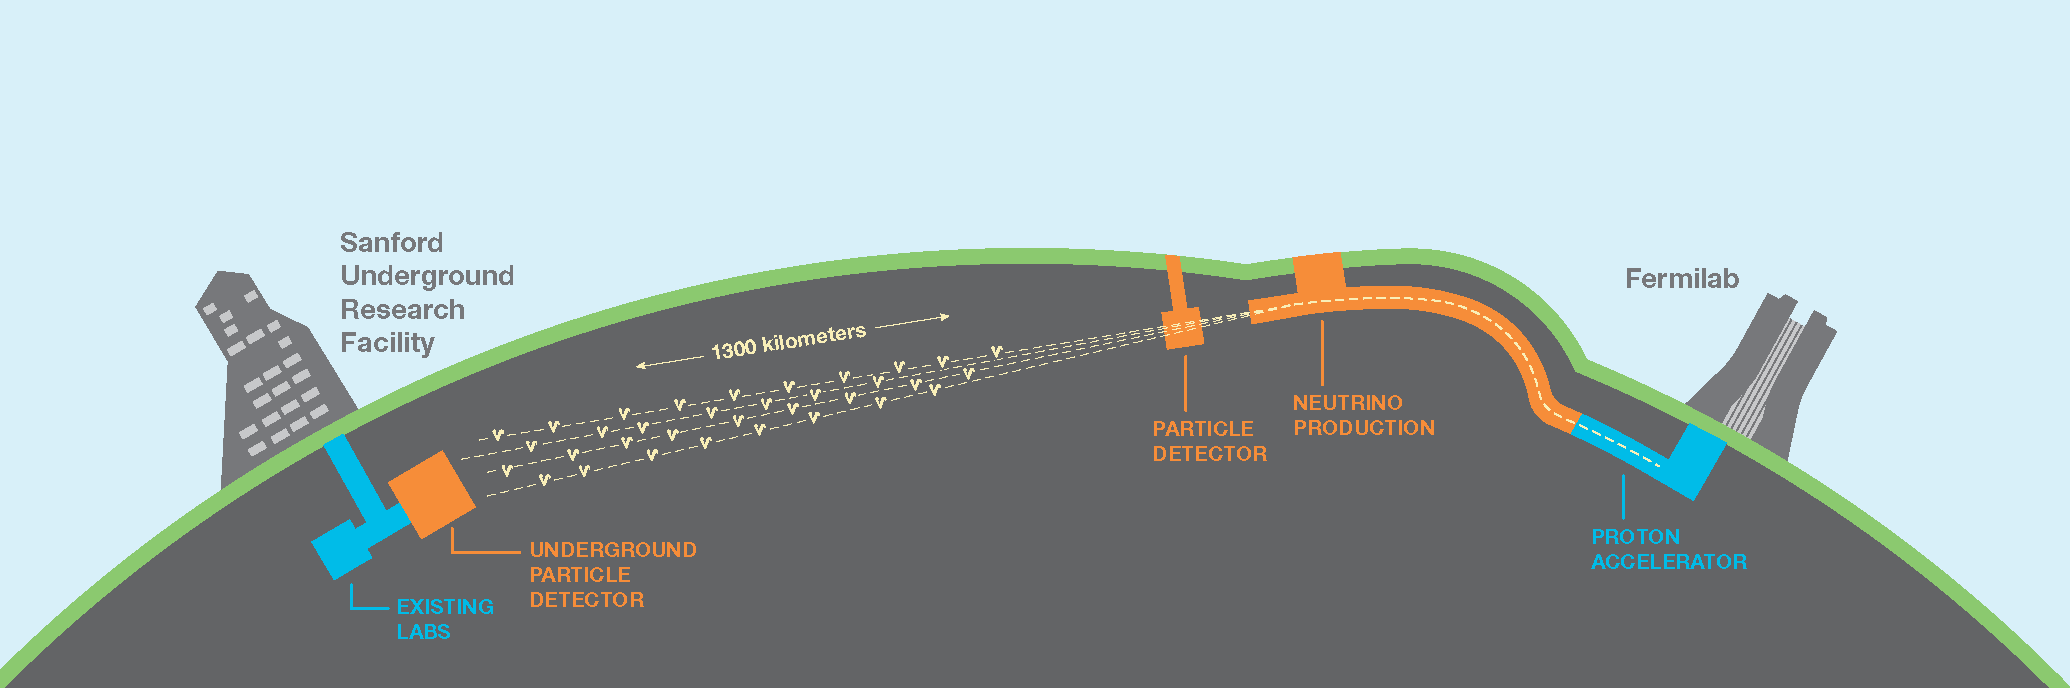
\includegraphics[width=\textwidth]{figures/dune_baseline.png}

	\caption
	[The Deep Underground Neutrino Experiment.]
	{The Deep Underground Neutrino Experiment. Figure from \cite{TODO}.}

	\label{fig:dune_baseline}

\end{figure}

The DUNE experiment will be a next generation neutrino physics and nucleon decay
experiment consisting of three principal components; an intense broad band 
neutrino beam and precise near detector based at the Fermilab National 
Accelerator Laboratory near Chicago, and a far detector at Sanford Underground 
Research Facility in South Dakota, approximately 1300 km away from the 
neutrino source, as demonstrated in Figure \ref{fig:dune_baseline}. The DUNE 
experiment identifies three primary scientific goals 
\cite{Abi:2020evt}:
\begin{itemize}
	\item Perform a comprehensive programme of neutrino oscillation measurements
		including measurements of \dcp{}, neutrino mass ordering, and the
		$\theta_{23}$ octant.
	\item Search for proton decay in several decay modes.
	\item Measure $\nu_e$ from a core--collapse supernova if one occurs within our
		galaxy during the lifetime of the experiment.
\end{itemize}
In addition, the experiment hopes to fulfill a significant programme of
secondary science goals:
\begin{itemize}
	\item Other accelerator based neutrino physics, such as non--standard
		interactions, sterile neutrinos, and CPT violation.
	\item Measurements of neutrino properties using atmospheric neutrinos.
	\item Dark matter searches in both the near and far detectors.
	\item A programme of neutrino interaction physics studies in the DUNE near
		detector.
\end{itemize}

To achieve these goals DUNE has opted to base the near and far detector designs
on the liquid argon time projection chamber (LArTPC) technology. The DUNE
far detector will consist of four LArTPC detectors each with 10 kt of active
liquid argon mass. This technology will have never before been used on this
scale, and therefore, there has been a significant programme of LArTPC research
and development ongoing to validate and characterise the performance of the 
technology for DUNE. 

\subsection{Liquid Argon Time Projection Chambers}
A LArTPC consists of a large volume of highly--purified liquid argon immersed in
an electric field. Charged particles traversing the liquid argon produce two
primary energy depositions, a trail of ionisation electrons along their path,
and prompt ultra--violet scintillation photons. After deposition the ionisation
electrons drift in the electric field toward the charge readout plane where they
induce electrical signals. Liquid argon is transparent to its own scintillation
light and therefore the scintillation photons can travel through the argon to be
collected in a photon detection system.The LArTPC detection principal is 
illustrated in Figure \ref{fig:lartpc}. 

\begin{figure}

	\centering

	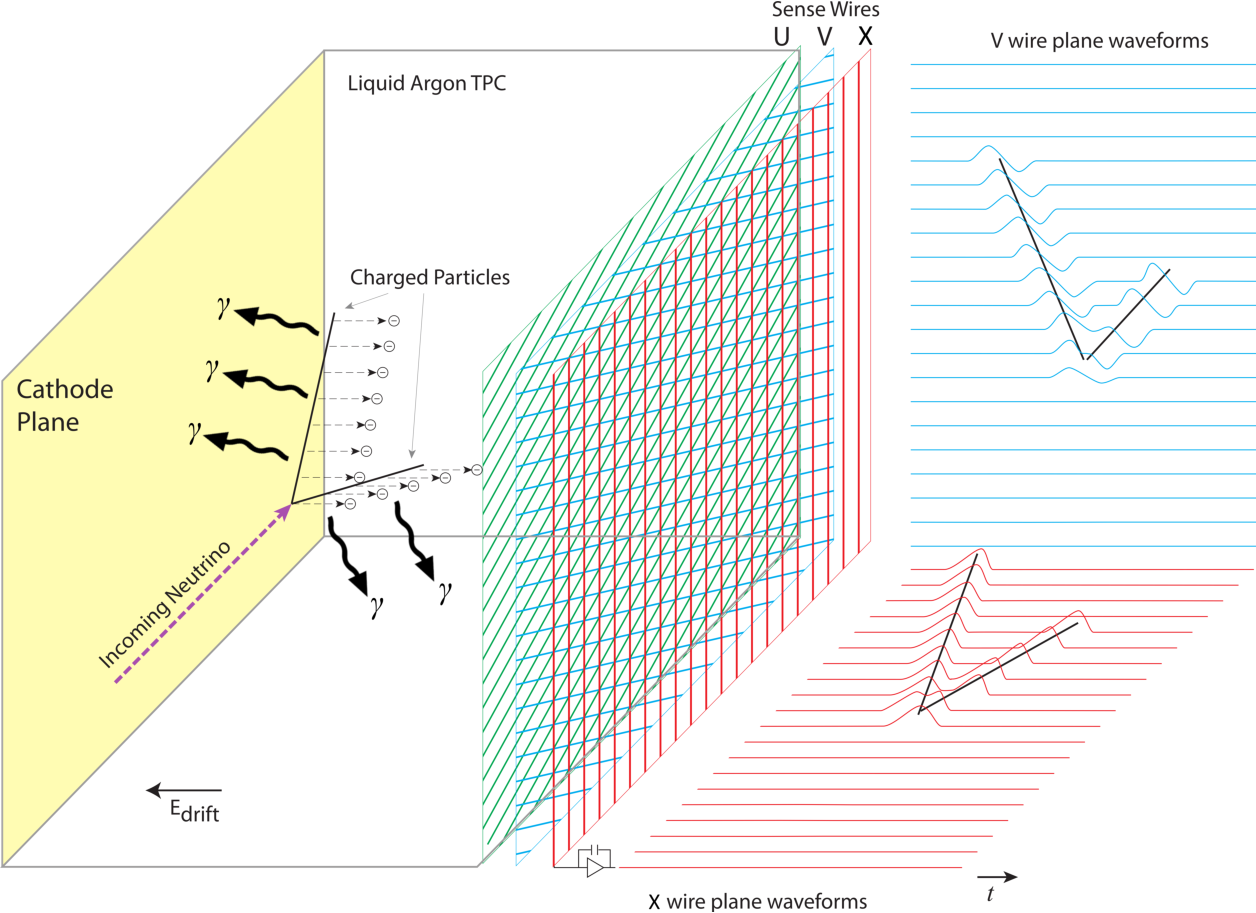
\includegraphics[width=\textwidth]{figures/LArTPC_Concept.pdf}

	\caption
	[LArTPC detection principal.]
	{LArTPC detection principal. Figure from \cite{Abi:2020loh}.}

	\label{fig:lartpc}

\end{figure}

The details of the charge readout and photon detection systems are specific to 
each detector, but broadly speaking LArTPC detectors can be split into two 
main categories: single--phase and dual--phase. In a single--phase detector the
drifting ionisation electrons remain in the liquid argon and the signals are 
typically read out on three anode wire planes. A dual--phase LArTPC contains an
additional region of gaseous argon in which a high electric field, known as the
extraction field, is applied to extract the ionisation from the liquid 
before it is amplified and collected on a pair of anode wire planes 
\cite{Abi:2020wmh}.

\bigskip

\protodune{} is one of two large scale prototypes for the DUNE far detector
modules, which focusses on the single--phase LArTPC technology. The DUNE far
detector modules feature a modular design in which each module is built up of a
number of identical components, \protodune{} was designed to prototype the
design of many of these components at a 1:1 scale, including the anode planes,
cathode plane, and photon detectors. The \protodune{} experiment has four 
primary goals, as outlined in the Technical Design Report \cite{Abi2017}:
\begin{itemize}
	\item Prototype the production and installation procedures for the
		single--phase far detector design.
	\item Validate the design from the perspective of basic detector performance;
		this can be achieved with cosmic-ray data. 
	\item Accumulate large samples of test-beam data to understand/calibrate the
		response of the detector to different particle species.
	\item Demonstrate the long-term operational stability of the detector as part
		of the risk mitigation program ahead of the construction of the first 10 kt
		far detector module.
\end{itemize}
As such, \protodune{} represents a significant milestone in the development of
the far detector for the DUNE experiment. Its successful operation, both in a 
test--beam and with cosmic rays, provides valuable data with which to understand
reconstruction and analysis of the data that will be collected by the DUNE far 
detector.

\section{The \protodune{} Detector} \label{sec:pdsp_detector}

The \protodune{} detector is located at the Neutrino Platform at CERN along the
H4 beam line. It is a single--phase LArTPC detector with a total liquid argon 
mass of 0.77 kt, making it the largest monolithic single--phase liquid argon TPC
to be built to date. The TPC comprises the following major components, which 
are illustrated in Figure \ref{fig:pdsp_tpc}:
\begin{itemize}
	\item A cathode plane constructed of modular Cathode Plane Assemblies (CPA).
	\item Two anode planes constructed of modular Anode Plane Assemblies (APA).
	\item A photon detection system (PDS) which is integrated into the APAs.
	\item A field cage (FC), beam plug, and high voltage systems (HV).
	\item Readout electronics submerged in the liquid argon, cold electronics 
		(CE). 
\end{itemize}
The detector components are designed to be an almost exact replica of the final 
single--phase far detector modules, but the detector has an overall scaling 
factor of approximately $1:20$ in terms of total liquid argon mass 
\cite{Abi2017}.

\begin{figure}

	\centering

	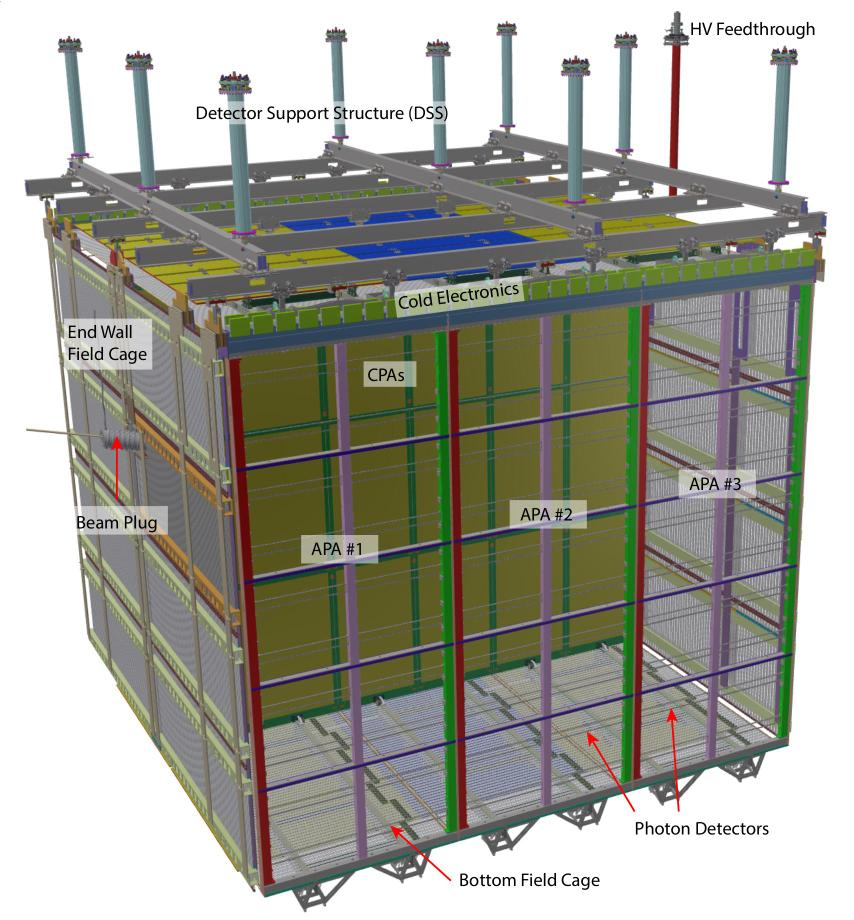
\includegraphics[width=0.9\textwidth]{figures/pdsp_tpc.jpg}

	\caption
	[The main components of the \protodune{} TPC.]
	{The main components of the \protodune{} TPC. Figure from \cite{Abi2017}.}

	\label{fig:pdsp_tpc}

\end{figure}

\subsection{The Liquid Argon TPC}

The \protodune{} TPC has an active volume of 6 m (height) $\times$ 7.2 m (width,
drift direction) $\times$ 7 m (length, approximate beam direction). The cathode 
plane at the center of the active width is flanked by two anode planes which 
define two 3.6 m drift volumes. The field cage around these two drift volumes
helps to ensure a uniform electric field within the drift region.

Each anode plane is modularly constructed from three APAs which have dimensions
6 m (height) $\times$ 2.3 m (width). The APA frame holds three sets of parallel
wires on the inward and outward facing sides, these are oriented at different 
angles to enable 3D reconstruction. The first two sets of wires are induction
wires, these are electrically connected and biased such that they are
electrically transparent to the drifting ionisation; ionisation passing the
induction wires causes an induced bi--polar signal. The third set of wires are 
known as collection wires, they are not electrically connected; when drifting 
ionisation approaches the collection wires it is absorbed producing a 
uni--polar signal. In \protodune{} each set of induction wires contains 800
wires at a 4.67 mm pitch, and each set of collection wires contains 480 wires at
a 4.79 mm pitch. The wire planes from each APA are read out by CE mounted on 
the APA frame. A total of 2560 electronics channels are used to read out the 
data from each APA.  The CE amplify and digitise the signals from the wires 
before transmitting them to the Data Acquisition System (DAQ).

The cathode plane in \protodune{} consists of an array of 18 CPA modules, 2 m 
(height) $\times$ 1.2 m (width). The cathode plane is held at -180 kV to 
provide a 500 $\mbox{Vcm}^{-1}}$ drift field in each of the drift volumes. The 
field cage surrounding the drift regions ensures that the electric field is 
uniform across the detector volume. \mccorrect{How does it do this? Equally
spaced resistors I think.}

One area in which the design of \protodune{} differs from the far detector is
the inclusion of the beam plug. This is necessary to minimize interactions
between the charged particle test--beam and the cryostat before the beam enters 
the active region of the detector. A cylindrical beam plug, containing 
nitrogen gas, penetrates from the cryostat wall into the field cage at 
location of the incoming test--beam \cite{TODO}. 

\subsection{The Photon Detection System}

In the single--phase far detector modules, the PDS must be embedded in the APA
frames. This is to maximise the light yield from scintillation, and to increase
the spacial information from the light by placing the photon detectors close to
the scintillation source.

\subsection{Cold Electronics and Data Acquisition}

\section{The H4 Beam Line} \label{sec:h4}


\section{Cosmic Rays in ProtoDUNE--SP} \label{sec:pdsp_cosmic}
\subsection{The Cosmic Ray Taggers}



\section{ProtoDUNE--SP Simulation and Reconstruction} \label{sec:pdsp_sim_reco}

\subsection{Simulation}

\subsection{Reconstruction}

\section{ProtoDUNE--SP Online Monitoring System} \label{sec:pdsp_om}


\chapter{\label{ch:4-energyloss}Energy Loss in Liquid Argon} 

\minitoc

This chapter will cover in more detail both the theory and measurement of
electromagnetic energy loss in liquid argon. Energy loss for both electrons and
photons will be discussed and the implications of this for electron
reconstruction at different energy scales will be highlighted. 

The work in this section is complete and part of this work was reported in the
document submitted for transfer of status.

\subsection{Electron Energy Loss}
\subsection{Photon Energy Loss}
\subsection{Electron--Ion Recombination}
\subsection{Implications on Electron Reconstruction in Liquid Argon}

\chapter{\label{ch:5-chargeid}Charge Identification with Convolutional Neural 
Networks} 

% \minitoc

\noindent A major problem faced by the next generation of neutrino experiments
is the correct categorisation of particle interactions within the detector.
Typically identifying the underlying type of a neutrino interaction involves
determining the lepton content of the final state particles; as such it is
important to be able to distinguish muons from electrons, or more generally
tracks from showers.

This chapter will describe an approach for hit classification in LArTPCs using
machine learning techniques. A brief theoretical overview of neural networks
will be presented in section \ref{ml}, including a discussion of convolutional
neural networks and their application to pattern recognition. Section
\ref{hit-id} will detail an approach to hit classification in LArTPCs based on
tagging the source of energy depositions with a convolutional neural network.
The performance of this approach will be analysed with ProtoDUNE--SP simulation
and data in sections \ref{cnn-perf-sim} and \ref{cnn-perf-data} respectively.

\section{Neural Networks} \label{ml}

An artificial neural network (ANN) consists of a set of nodes, together with a
set of connections between those nodes. The nodes in the graph take the form of
an artificial neuron which passes a number of inputs through a nonlinear
activation function to produce a single output. In an ANN the connections
provide a mechanism for taking the output of a given node and using it as the
input for a subsequent node. This structure of nodes and connections provides a
very flexible framework, the basis for a number of machine learning algorithms
which utilise this flexibility to learn the structure of complex data sets.

In order for an ANN to make accurate predictions based on data, the weights and
biases between each set of neurons must be tuned such that the outputs of the
network match those expected for a given input. In supervised learning
\cite{Reed:1998:NSS:552600}, the loss, a measure of the difference between the
truth and the output of an ANN, can be used to learn the appropriate values of
the weights and biases using the method of gradient descent. The loss is
computed and its gradient as a function of the weights and biases can be
calculated with the back--propagation algorithm \cite{Rumelhart1986}; the loss
is then minimised based on the gradient calculated with back--propagation. This
process can be repeated until the loss function reaches an acceptable level or
stops decreasing.

One of the most widely used ANN's is the multi--layer perceptron (MLP)
\cite{Reed:1998:NSS:552600}; this class of networks consists of at least three
layers of nodes: an input layer, one or more hidden layers, and an output layer.
These layers are connected in a feed--forward configuration such that the graph
of nodes contains no cycle. Traditionally, the layers are also fully connected
such that the output of each node is connected to the inputs of all nodes in the
next layer. These networks are able to approximate any function to arbitrary
precision with a single hidden layer \cite{Cybenko1989ApproximationBS}; however,
there is no limit on the number of nodes required in order to achieve a good
approximation. In practice networks with additional hidden layers can reach the
required precision with fewer nodes than a network with a single hidden layer
\cite{Lecun2015}.

ANN's provide a flexible tool for a variety of pattern recognition tasks but
there can be issues with their training and use. Typical issues with ANN's
include a risk of slow learning due to vanishing gradients for typical sigmoid
activation functions and a high risk of over--training due to the large number
of free parameters. In particular, over--training can lead to poor
generalisation of the network for real world examples, despite excellent
performance when evaluated on the training sample \cite{Reed:1998:NSS:552600}.

An extension of the MLP with considerable success, particularly in image
classification tasks, is the convolutional neural network (CNN)
\cite{Jackel2008, Szegedy2015}. When evaluating data with a high dimensional
input, having a fully connected network architecture leads to large numbers of
neurons and high computational cost. In addition, for spatially correlated data
such an architecture does not take the local spatial structure of the data into
account. A CNN attempts to resolve these issues by exploiting the local
connectivity of the data; single input neurons are replaced by convolutional
kernels which are evaluated on small regions of the input. These convolutional
kernels are evaluated over all valid locations in the input producing feature
maps which describe the spatial distribution of the features which each kernel
has learned to identify. Each set of feature maps can then be used as an input
for either convolutional layers or fully connected layers. 

Convolutional kernels provide a local translation invariant evaluation of
features within the data; with this method low level features are identified
first and their spatial distribution can then be exploited to identify higher
level structure in the data \cite{Jackel2008}. This makes these networks ideal
for pattern recognition in images, where common features can be located anywhere
in the image. The high spatial and calorimetric energy resolution of LArTPC
detector data make these algorithms an ideal candidate for classification of the
data, and successful applications on CNNs have been achieved in ongoing neutrino
experiments \cite{Aurisano:2016jvx, Acciarri:2016ryt}. The remainder of this
chapter will detail a use of CNNs to identify low level features in LArTPC data.

\section{Hit Identification with Convolutional Neural Networks}
\label{hit-id}

As well as in neutrino event classification, effective track shower separation
has important applications throughout DUNE's physics programme; defining pure
calibration samples such as minimum ionising muons and \(\pi_0\) decays is
crucial for understanding the energy response of the DUNE detector. Each of
these samples has a unique topology, but the first step in identifying many of
these samples is the same: defining tracks and showers which can be combined to
give the final state. To do this collections of hits have to be clustered and
identified as track or shower objects. Here we will present a method for
classifying the ionisation source of hits, a label is then associated with each
hit, and subsequent reconstruction and analysis algorithms can use this when
defining data samples.

Aside from track and shower objects, a useful calibration sample with a unique
topology in LAr is the Michel electron. At typical Michel electron energies the
ionisation energy loss of electrons in LAr undergoes a transition from collision
dominated to radiation dominated, as such Michel electrons typically have a
combined topology with a short track--like component and a few small radiated
energy depositions. Due to the unique topology of these interactions, Michel
electrons where chosen as a unique category for hit classification. 

A CNN was used for hit classification, the network was trained to predict
\(\{p_t, p_s, p_e, p_m\}\), the probabilities for track, shower, empty, and
Michel classifications respectively. The empty category is included to ensure
that the network doesn't learn to assign a track--like or shower--like tag to
empty or noisy regions of the data. Since the Michel electron category has
overlap with the track and shower categories, the Michel electron probability is
decoupled from the other probabilities which are constrained to sum to one.

Training data was built using simulations of the ProtoDUNE--SP detector in the
LArSoft framework \cite{Snider2017}; cosmic ray simulations were combined with
simulations of the ProtoDUNE--SP beam for peak beam energies in the range 1--7
GeV and both positive and negative beam polarity. The input was formed of small
patches of the raw detector readout in each plane, 48 wires in total where
considered around the central energy deposition and an equal number of bins were
formed in the drift time coordinate by averaging the ADC values over time such
that the distance scale was equal in both coordinates. The truth for each
training sample was obtained from the simulation by associating the measured
ionisation energy depositions to the corresponding simulated particle. In total
\(\sim26\) million input patches were produced, figure \ref{fig:patches} shows
example patches for each label type, and details of the number of each patch
type in the training, validation, and test data sets are given in table
\ref{tab:patches}. 

\begin{figure}[h]
	\centering
	\includegraphics[width=0.5\textwidth]{figures/patch_examples.pdf}  
	\caption[Example CNN input images.]{Example input patches for
	each label. Clockwise from top--left: Shower, Track, Empty, Michel.}
	\label{fig:patches}
\end{figure}

\begin{table}[h]
	\centering
	\begin{tabular}{c|c|c|c|c}
		Patch Type & Shower     & Track     & Empty     & Michel  \\ \hline
		Training   & 13,493,982 & 9,727,604 & 2,517,882 & 731,456 \\
		Validation & 734,673    & 562,038   & 141,388   & 42,727  \\
		Test       & 764,659    & 518,805   & 139,987   & 39,674 
	\end{tabular}
	\caption[Number of patches with each truth label.]{Summary of the number of
	samples with each truth label in the training, test, and validation data
	sets.}
	\label{tab:patches}
\end{table}

The network architecture was designed to provide the best performance possible
given constraints on running time; since the CNN is part of the low level
reconstruction chain and it must run over a large number of candidate images for
each event, run time for each event is required to be \(O(10)\)s. While better
classification performance was achieved with deeper networks, the best
performance while achieving the running time goal was achieved with a relatively
shallow network consisting of one convolutional layer followed by two dense
layers; it is reasonable to assume that with improved computational resources,
e.g. evaluation with GPU's, the performance of the classification could be
improved within the time constraints. 

The TensorFlow library was used to design and train the CNN, with the
TensorBoard visualisation suite being used to monitor training \cite{45381}. The
final network architecture used is shown in figure \ref{fig:arch}; the
\(48\times48\) pixel input images are passed through a single convolutional
layer with 48 \(5\times5\) filters; the output feature map is passed onto a pair
of dense layers with 128, and 32 nodes respectively. Leaky rectified linear
units are used as activation functions throughout the hidden layers
\cite{He2015}. These units are more computationally efficient than sigmoid like
functions as well as providing a non--vanishing gradient for all inputs,
avoiding saturation in learning. The output of the network is split into two
branches; a three--way softmax function is used to constrain the joint
probability for track, shower, and empty to sum to one, and a sigmoid function
is used for the output of the Michel electron classifier. Finally,
regularisation is achieved with the dropout algorithm
\cite{Srivastava2014DropoutAS}; in each iteration of the training weights have a
probability \(p\) to be set to zero while the remaining weights are scaled by a
factor \(1/(1-p)\). With this approach, each training iteration uses only a
random sample of the available nodes and as such nodes cannot co--adapt. The
resulting network is a model average of each possible sub--network.

\begin{figure}[h]
	\centering
	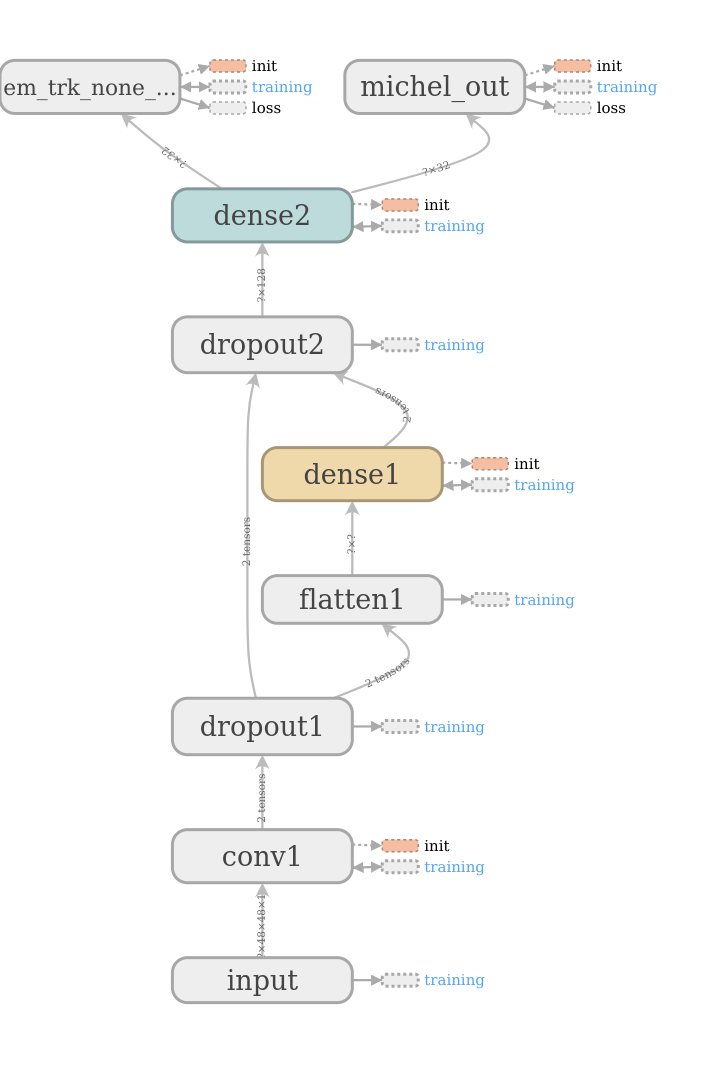
\includegraphics[width=0.6\textwidth]{figures/network_graph.png}
	\caption[Network architecture used for hit classification.]{Network
	architecture used for hit classification, visualisation from the TensorBoard
	library.}
	\label{fig:arch}
\end{figure}

The network was trained using stochastic gradient descent (SGD) with the total
loss being the weighted sum of the losses for the two output branches, \(L_{tot}
= 0.1 \cdot L_{tse} + L_m\), where the Michel classifier is given higher
precedence due to the smaller training data set available for the Michel output.
In order to speed up the learning process and converge on an optimal model, both
the momentum and decay algorithms were used; momentum reduces oscillations of
the weights during learning, while the decay of the learning rate allows for
rapid learning during early stages of SGD and increased precision as the model
converges \cite{Reed:1998:NSS:552600}. Learning metrics were monitored during
training using TensorBoard. The losses for each branch as well as the total loss
for the validation data set are given in figure \ref{fig:training} as a function
of the training epoch. The validation losses remain stable giving an indication
that regularisation with dropout was successful in preventing over--fitting of
the training data. However, the validation set loss does not increase
significantly after the first couple of epochs and so the training could have
been terminated sooner with this network architecture. The final losses measured
with the test data set are given in table \ref{tab:losses}. 

\begin{figure}[h]
	\centering
	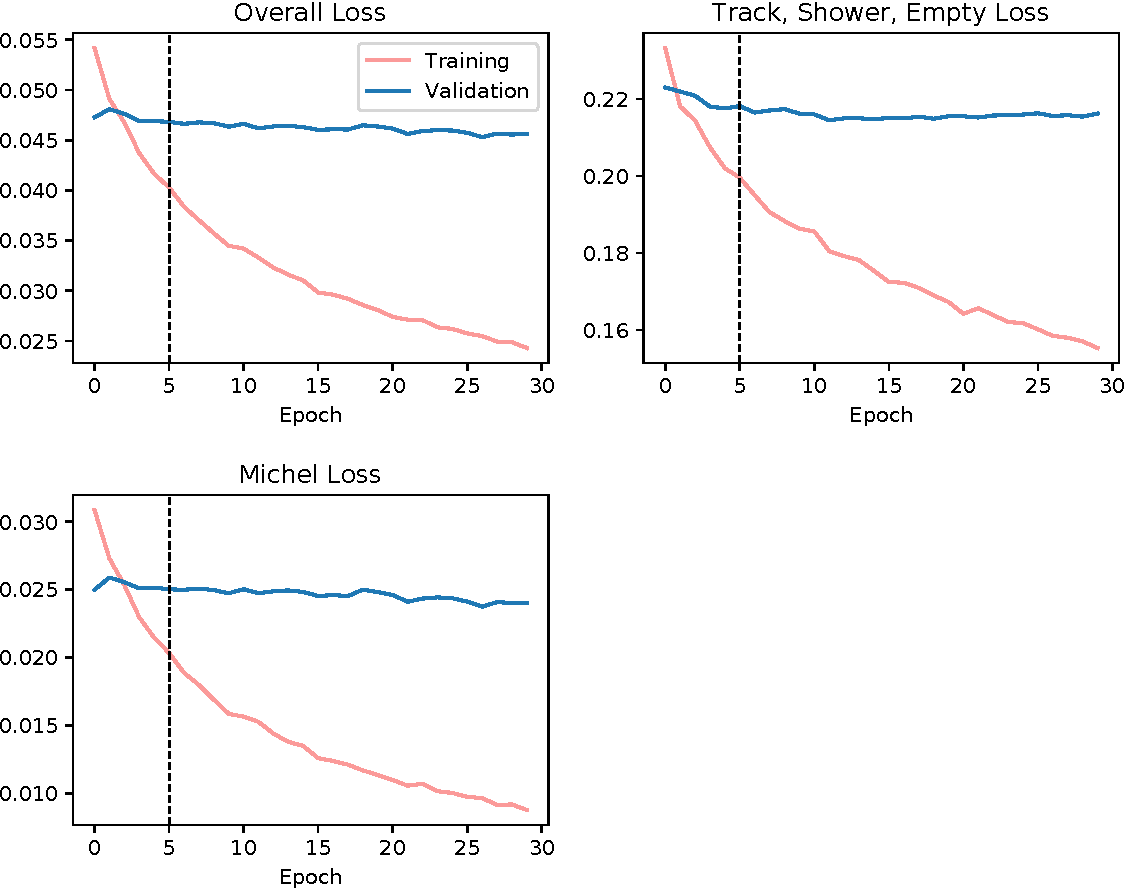
\includegraphics[width=\textwidth]{figures/losses_prelu.pdf}
	\caption[Validation and training set losses.]{Evolution of the validation
	and 
	training set losses during the training process.}
	\label{fig:training}
\end{figure}

\begin{table}[h]
	\centering
	\begin{tabular}{c|c|c|c}
		Loss Type   & \(L_{tot}\) & \(L_{tse}\) & \(L_m\) \\ \hline
		Loss Value  & 0.033       & 0.155       & 0.017   \\
	\end{tabular}
	\caption[Test set losses.]{Test set losses after full training process.}
	\label{tab:losses}
\end{table}

\section{Performance on ProtoDUNE--SP Simulation} \label{cnn-perf-sim}

The performance of the hit tagging was evaluated with reconstructed events in
the ProtoDUNE--SP detector from the latest simulation samples; in the
simulations, the detector was simulated under a number of different conditions,
specifically including the space charge effect (SCE) \cite{Mooney:2015kke} and
excluding it. The hit tagging was trained on a part of the simulated data set
which included the SCE and, as such, the samples without the SCE can be used as
a validation that the network is robust to SCE differences between the
simulations, and hence between the simulations and the data.

The distributions of the shower like classifier output for true shower hits and
all other hits are given in figure \ref{fig:show_output}; a strong separation
between track and shower hits is observed. The shower classification threshold
was optimised based on the F1 metric. This metric is defined as the harmonic
mean of the precision and recall of a classifier and optimising with this score
will ensure that both precision and recall will be high in the final classifier;
for use cases where neither precision or recall is favoured, the F1 metric can
be used to optimise for the best overall performance. The value of the F1 metric
as a function of threshold is also shown in figure \ref{fig:show_output}; the
score peaks at a threshold of 0.72 with a value of 0.863 corresponding to a
precision of 0.863 and a recall of 0.863.  

\begin{figure}[h]
	\centering
	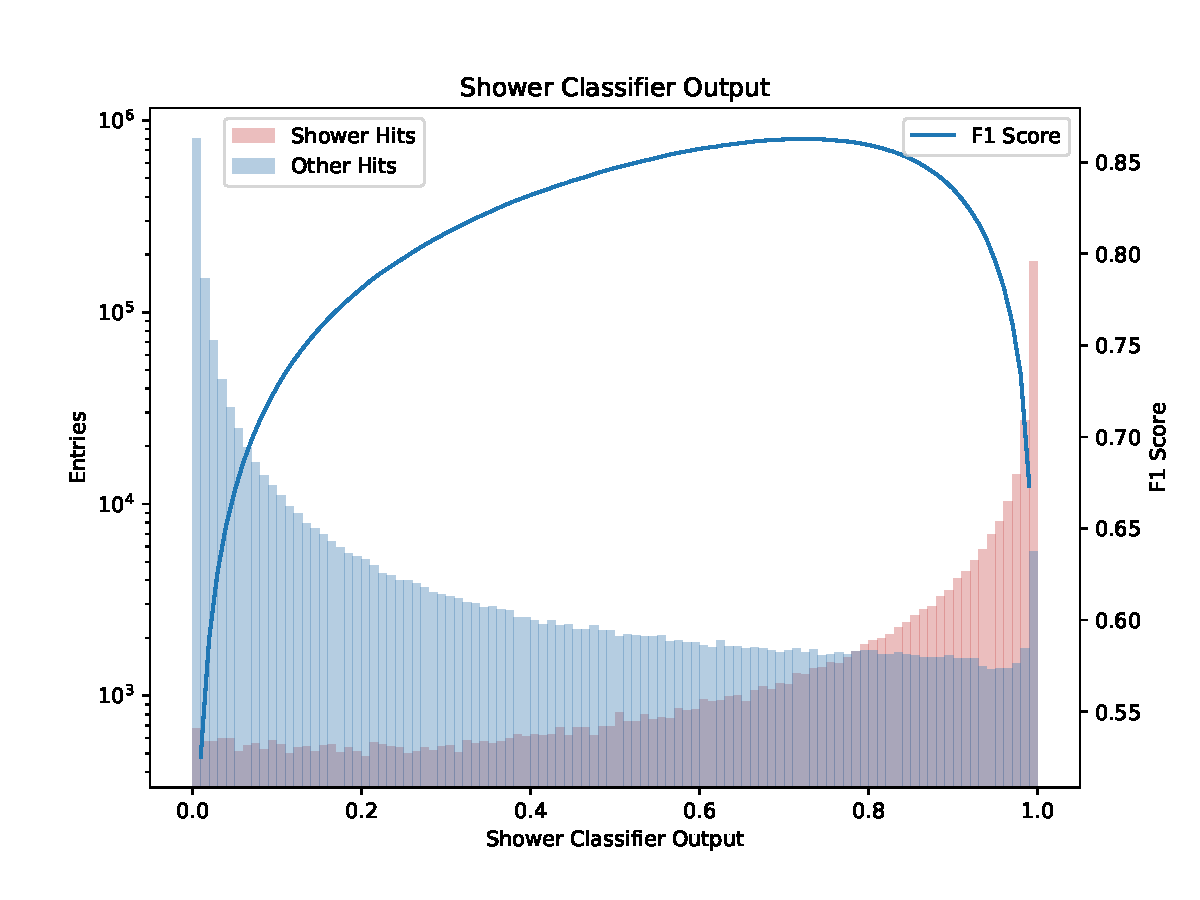
\includegraphics[width=0.8\textwidth]{figures/shower_combined.pdf} 
	\caption[Shower classifier output distributions.]{Shower classifier output
	distributions for true showers, and all other hits. Threshold optimisation
	was
	done using the F1 score metric which is also plotted.}
	\label{fig:show_output}
\end{figure}

Figure \ref{fig:michel_output} gives the distributions of the Michel classifier
output for true Michel electrons and all other hits. The large difference in
sample size between the Michel electron and other hits in this sample means that
despite high recall by the Michel electron classifier, low precision is
achieved. In chapter \ref{ch:6-michel} we will see that despite the low
performance of the classifier for individual hits, a pure sample of Michel
electron events can be selected by clustering hits with high Michel electron
scores. This is due to the fact that the simple hit by hit classification test
does not account for spatial correlations between Michel tagged hits.

\begin{figure}[h]
	\centering
	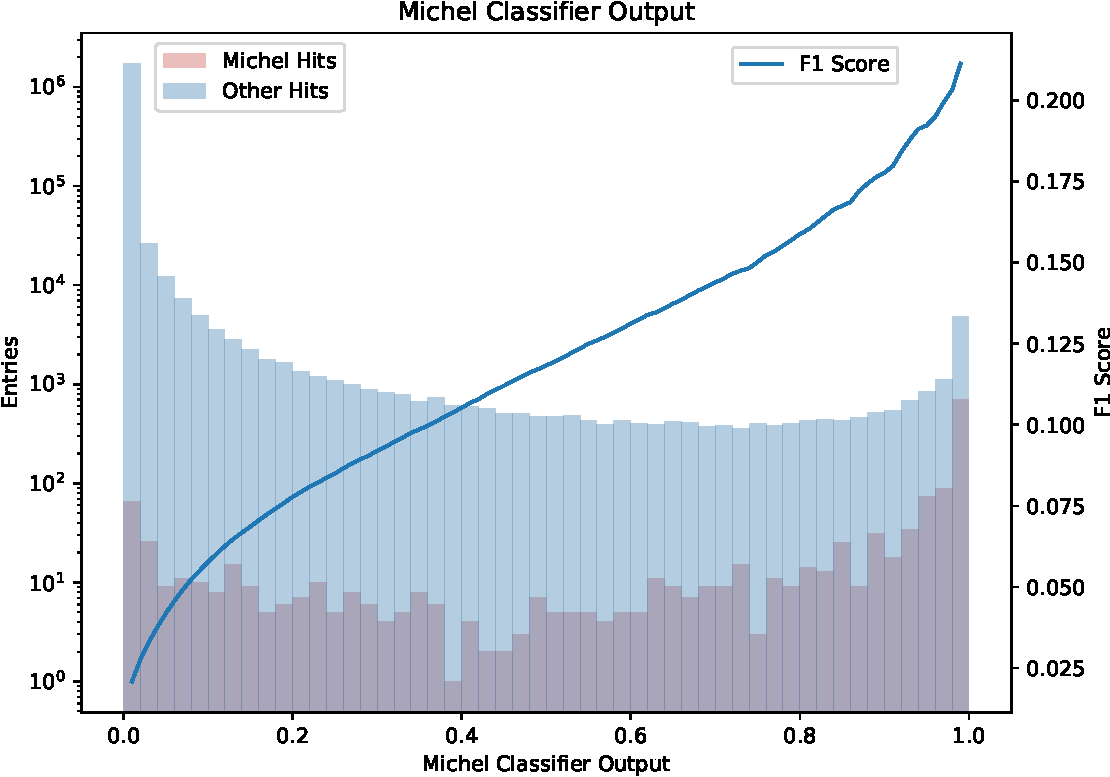
\includegraphics[width=0.8\textwidth]{figures/michel_combined.pdf} 
	\caption[Michel classifier output distributions.]{Michel classifier output
	distributions for true Michel electrons, and all other hits. Threshold
	optimisation was initially done with the F1 score metric, the threshold was
	modified when combined with a clustering algorithm, see chapter
	\ref{ch:6-michel}.}
	\label{fig:michel_output}
\end{figure}

Finally, the overall performance of each classifier was evaluated using the
receiver operating characteristic (ROC) curve \cite{Fawcett2006}; ROC curves are
a test of the classification ability of a binary classifier. The curves show a
comparison of the true positive rate and the false positive rate of the
classifier as a function of the classification threshold chosen for the
classifier. Figure \ref{fig:show_roc} shows the ROC curves for the shower and
Michel classifiers; the locations of these curves in the top left corner of the
plots show that both have excellent performance as classifiers. In addition, the
ROC curves show good agreement between the SCE on and SCE off data sets, showing
that the classifiers are robust to changes in the SCE model should it differ
between data and simulation. It is worth noting that the ROC curve only accounts
for classification rates within each true sub--sample, it cannot account for the
difference in sample size between the Michel electron sample and all other hits,
and thus the ROC curve is a more instructive metric for the shower classifier
where the size of the true and false samples are of a similar magnitude.

\vspace{-5mm}

\begin{figure}[h]
	\centering
	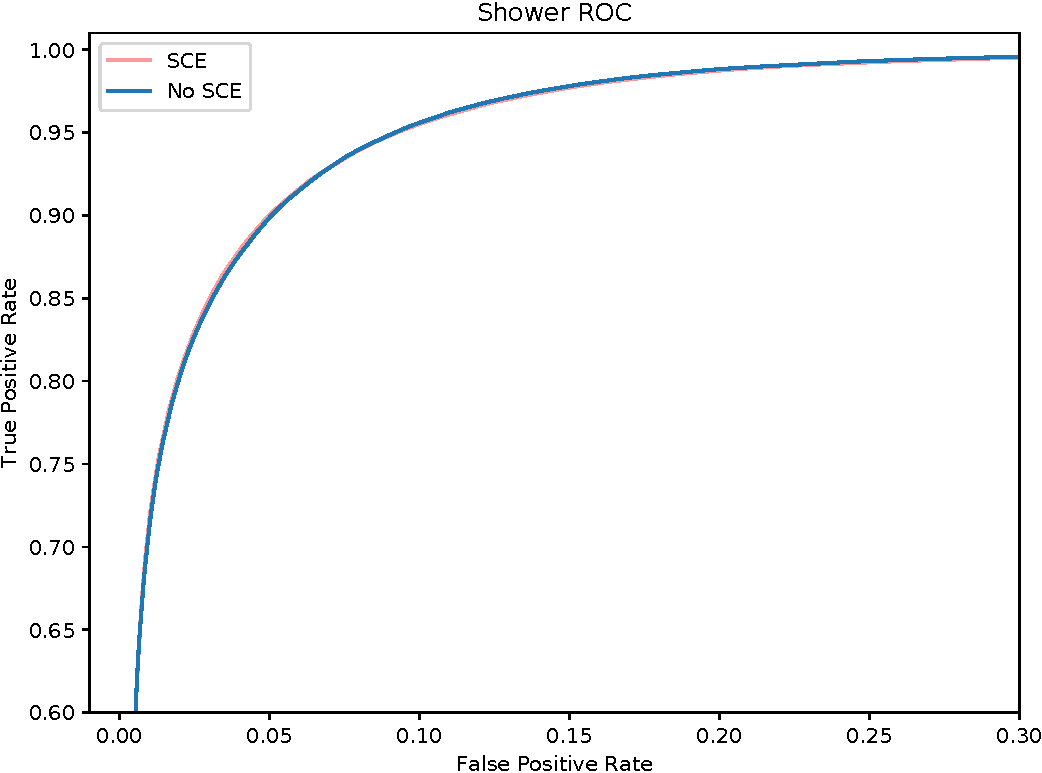
\includegraphics[width=0.65\textwidth]{figures/show_roc_comparison.pdf}
	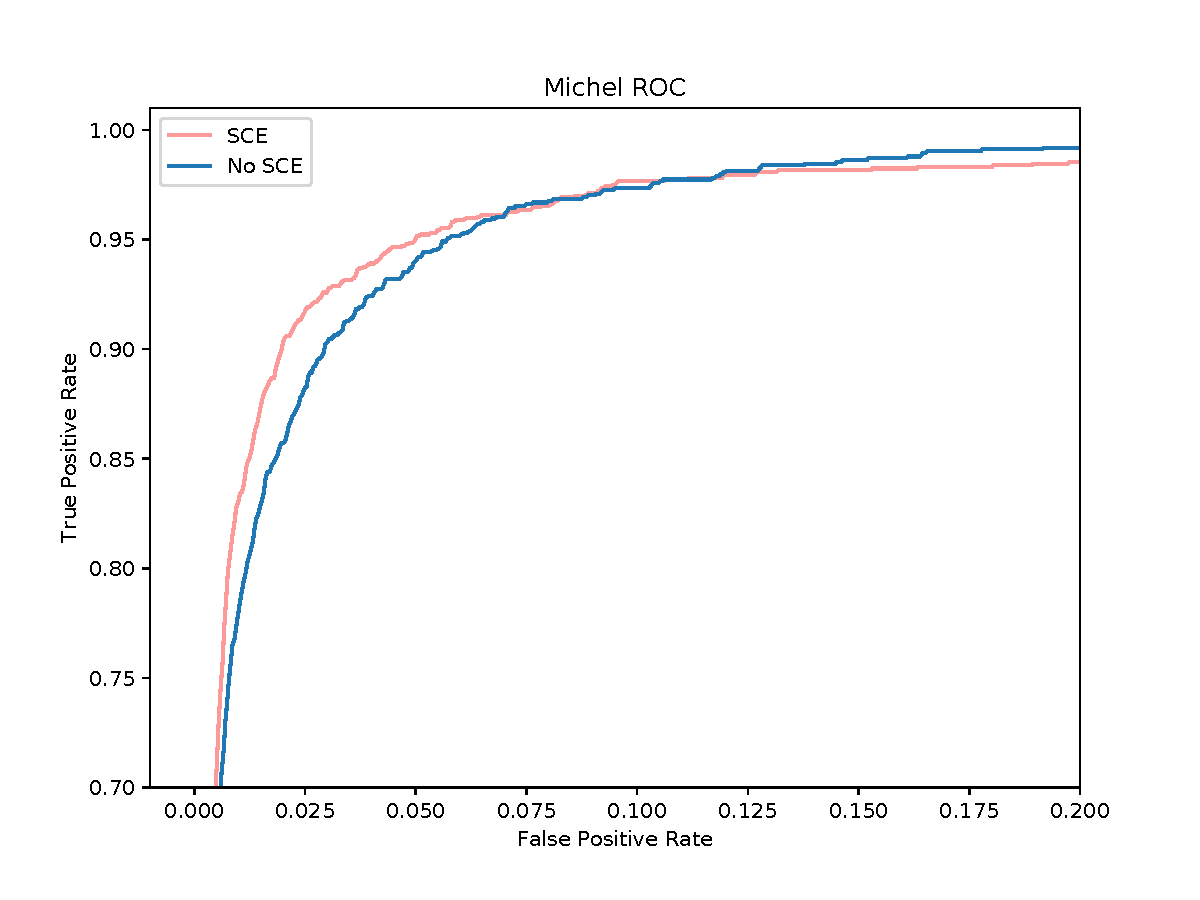
\includegraphics[width=0.65\textwidth]{figures/michel_roc_comparison.pdf}
	\caption[ROC curves.]{ROC curves for the shower (top), and Michel (bottom)
	classifiers. ROC curves for simulations including and excluding the SCE are
	included.}
	\label{fig:show_roc}
\end{figure}

\section{Validation and Performance on ProtoDUNE--SP Data}
\label{cnn-perf-data}

For validation on real ProtoDUNE--SP data two approaches were used: visual
validation with event scans and cross validation with the output of the Pandora
reconstruction framework \cite{Marshall2015}. Data from ProtoDUNE--SP run number
5387 was used for the validation; the data for this run was taken under stable
operating conditions with a peak beam energy of 1 GeV. 

Hand scans of the events show qualitatively that performance on the data is
good. Figure \ref{fig:real_event} shows an example of the track like
classification of hits in a real event. We can see that for hits along the
tracks the classifier produces a large output score, and for shower like
activity in the event the score is low, as we expect. In particular the
classifier is able to identify that hits which are adjacent to the track, delta
rays, are from scattered electrons.

\begin{figure}[h]
	\centering
	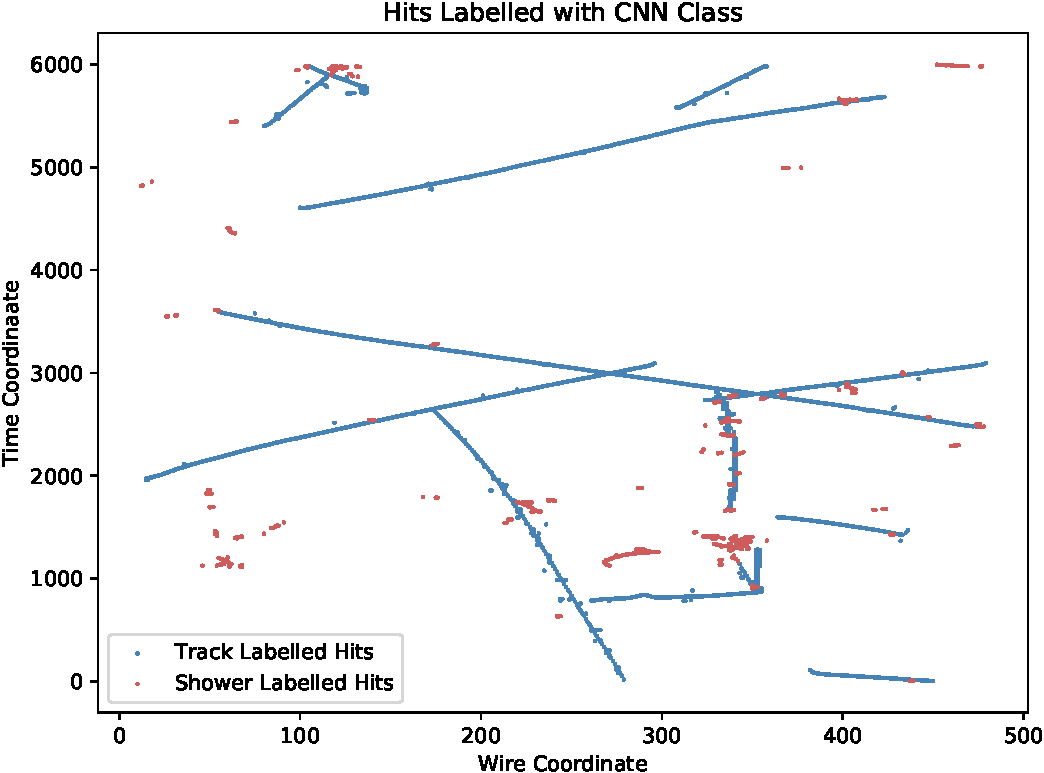
\includegraphics[height=0.45\textheight]{figures/track_score.pdf}
	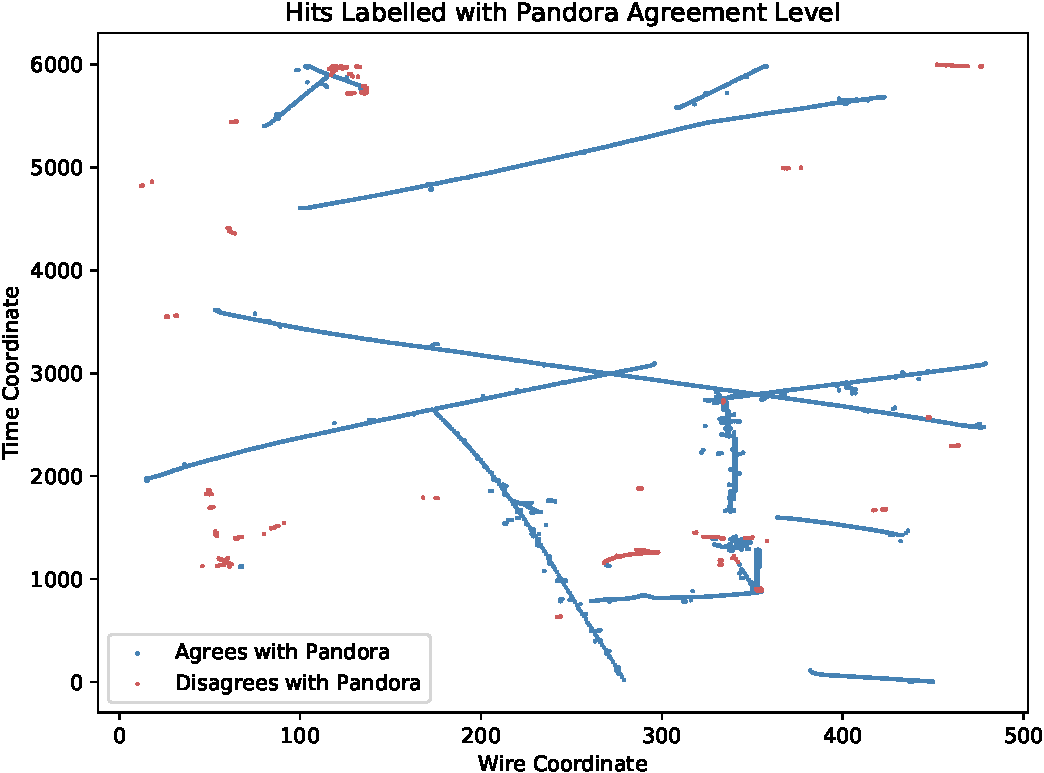
\includegraphics[height=0.45\textheight]{figures/pandora_agreement.pdf} 
	\caption[CNN output on an event from ProtoDUNE--SP data.]{Reconstructed
	hits from ProtoDUNE--SP run number 5387 labelled with CNN classification
	(top), and Pandora agreement level (bottom).}
	\label{fig:real_event}
\end{figure}

The Pandora reconstruction framework is the primary reconstruction used by the
ProtoDUNE--SP experiment; for a more quantitative validation of the performance
of the hit tagging algorithm, the hit tagging output can be compared to the
reconstructed objects produced by Pandora. After the ProtoDUNE--SP data has been
reconstructed, all of the reconstructed hits will have been clustered into
either track or shower objects. As such the comparison of a hits CNN output with
the type of reconstructed object it belongs to is a test of the agreement
between the CNN approach and the Pandora reconstruction algorithms. The Michel
electron performance cannot be validated in this way due to a lack of tagged
Michel electron objects in the Pandora output. Therefore, hand scanning of
events is the primary validation of the Michel electron classifier and will be
discussed in chapter \ref{ch:6-michel}.

The first test performed was the comparison of the CNN output distributions for
hits in both Pandora tracks and Pandora showers, the corresponding distributions
are given in figure \ref{fig:pandora} for both data and Monte Carlo; a strong
correlation between the reconstructed Pandora objects and the associated CNN
score can be seen in both cases, however the correlation is stronger in Monte
Carlo than in data. The discrepancy between Pandora and the CNN is still being
understood, differences between the data and simulations impact the performance
of both algorithms. Figure \ref{fig:real_event} shows reconstructed hits
labelled according to whether they agree or disagree with Pandora, we can see
that for long tracks the agreement is good while smaller objects tend to
disagree, with the CNN typically assigning a shower like classification but
Pandora reconstructing them as a track. Work to understand the discrepancy
between the CNN score and Pandora is ongoing.

\begin{figure}[h]
	\centering
	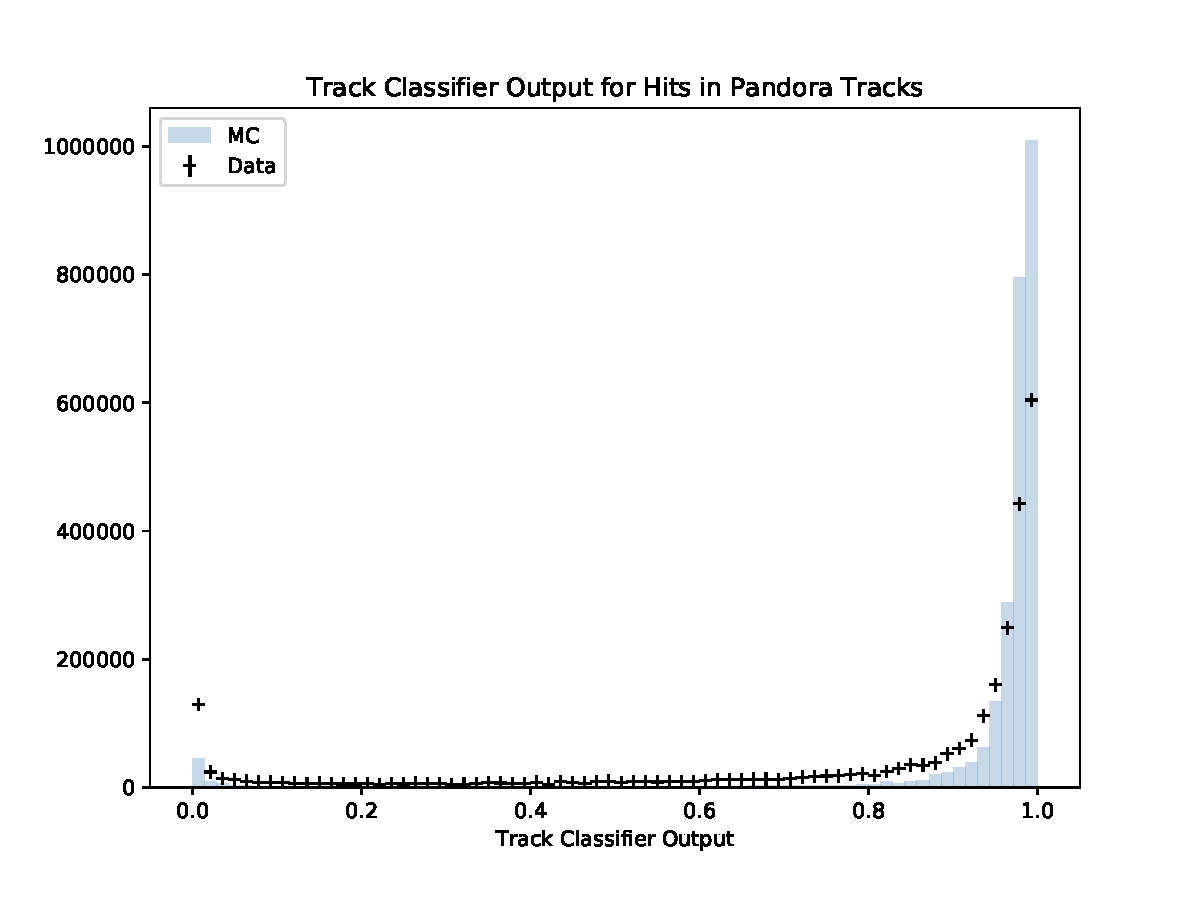
\includegraphics[width=0.7\textwidth]{figures/track_data_v_mc.pdf}
	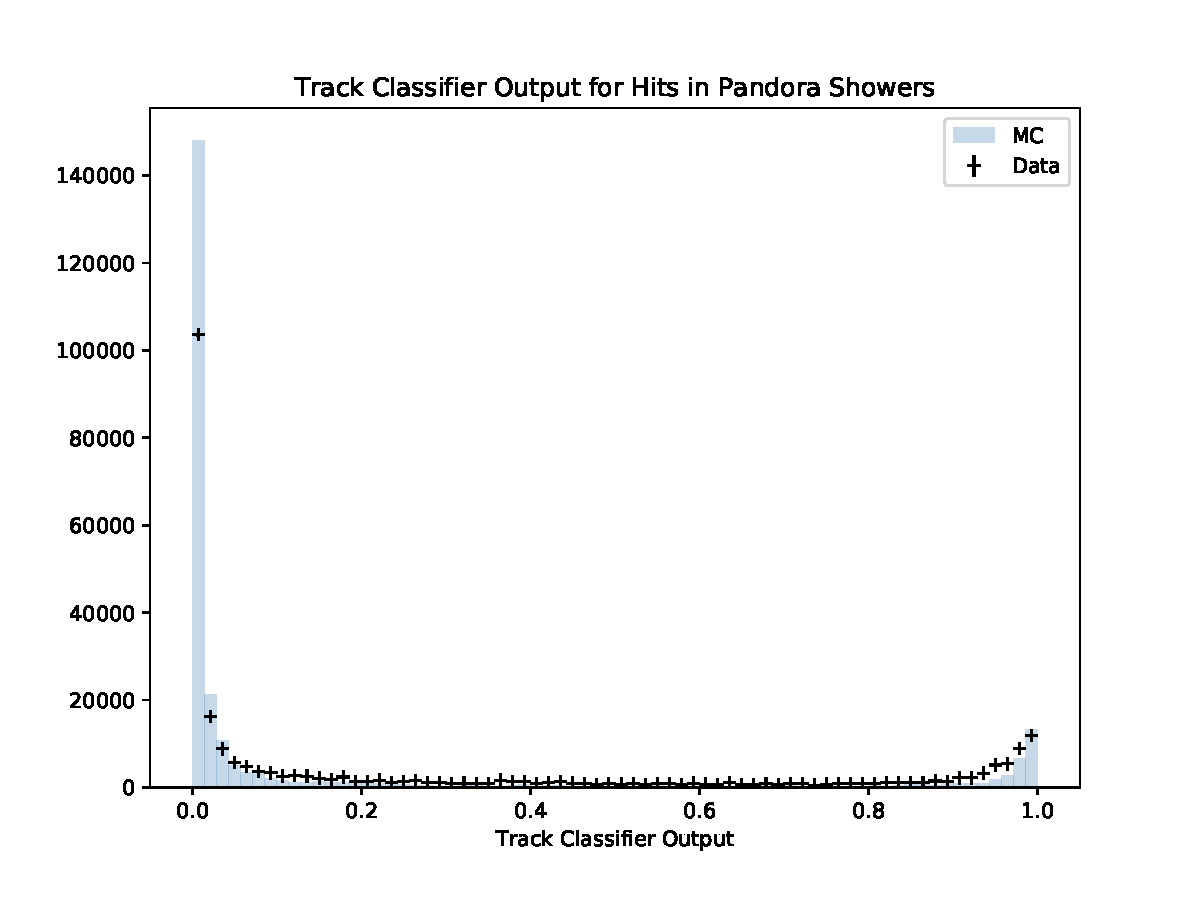
\includegraphics[width=0.7\textwidth]{figures/shower_data_v_mc.pdf}
	\caption[Output distributions for the track classifier on reconstructed
	Pandora objects.]{Output distributions for the track classifier on
	reconstructed Pandora objects.} \label{fig:pandora}
\end{figure}

This chapter has presented work on the development of a hit classification
algorithm for LArTPCs based on CNNs; the performance of this approach for
track--shower separation has been evaluated with ProtoDUNE--SP simulation and
reconstruction, demonstrating good performance. This hit tagging framework is
designed such that it can be utilised throughout the LArSoft reconstruction
chain and is complementary to other reconstruction algorithms in the framework;
chapter \ref{ch:6-michel} will detail an example use of the hit tagging output:
Michel electron event selection.

\noindent Additional plans for this chapter are detailed below.
\begin{itemize}[noitemsep,nolistsep]
	\item Understand the difference between data and MC when comparing the
	CNN to Pandora.
	\item Test network robustness to other detector effects in
	simulation. 
	\item Retrain networks with future simulations, including data
	driven models of detector effects.
\end{itemize}


\chapter{\label{ch:6-michel}Study of Michel Electrons in \protodune{}} 

\minitoc

%%%%%%%%%%%%%%%%%%%%%%%%%%%%%%%%%%%%%%%%%%%%%%%%%%%%%%%%%%%%%%%%%%%%%%%%%%%%%%%%
% FROM COS
%
% This chapter will cover the primary analysis of this thesis; a study of Michel
% electrons in the ProtoDUNE--SP detector which aims to investigate the agreement
% between data and simulation, and to provide an estimate of the energy scale
% uncertainty and energy scale bias for electrons in the 0--60 MeV range. 
% 
% The work done for this section is ongoing; preliminary work on this topic was
% presented in the report submitted for transfer of status. The rest of the work
% for this section is expected to be completed by the end of October 2019.
% 
% \noindent The work done as of writing for this chapter is as follows:
% \begin{itemize}[noitemsep,nolistsep]
% 	\item Event selection algorithm developed based on clustering of the Michel
% 	like hits discussed in the previous chapter.
% 	\begin{itemize}[noitemsep,nolistsep]
% 		\item Purity of > 98\% and efficiency of 5\% measured in ProtoDUNE--SP 
% 		simulations.
% 	\end{itemize}
% 	\item Two possible energy reconstruction algorithms developed.
% 	\begin{itemize}[noitemsep,nolistsep]
% 		\item Cone algorithm.
% 		\item Semantic segmentation algorithm with U-ResNet CNN architecture.
% 	\end{itemize}
% \end{itemize}
% 
% \noindent The work left to do is as follows:
% \begin{itemize}[noitemsep, nolistsep]
% 	\item Validation of algorithms on the real ProtoDUNE--SP data.
% 	\item Data MC comparison for Michel electron energy spectrum.
% 	\item Energy scale uncertainty and energy scale bias measurements with 
% 	measured Michel electron energy spectrum.
% \end{itemize}
% 
% \noindent An example Michel electron candidate event from the real ProtoDUNE--SP 
% data is given in figure \ref{fig:michel_event}.
% 
% \begin{figure}[h]
% 	\centering
% 	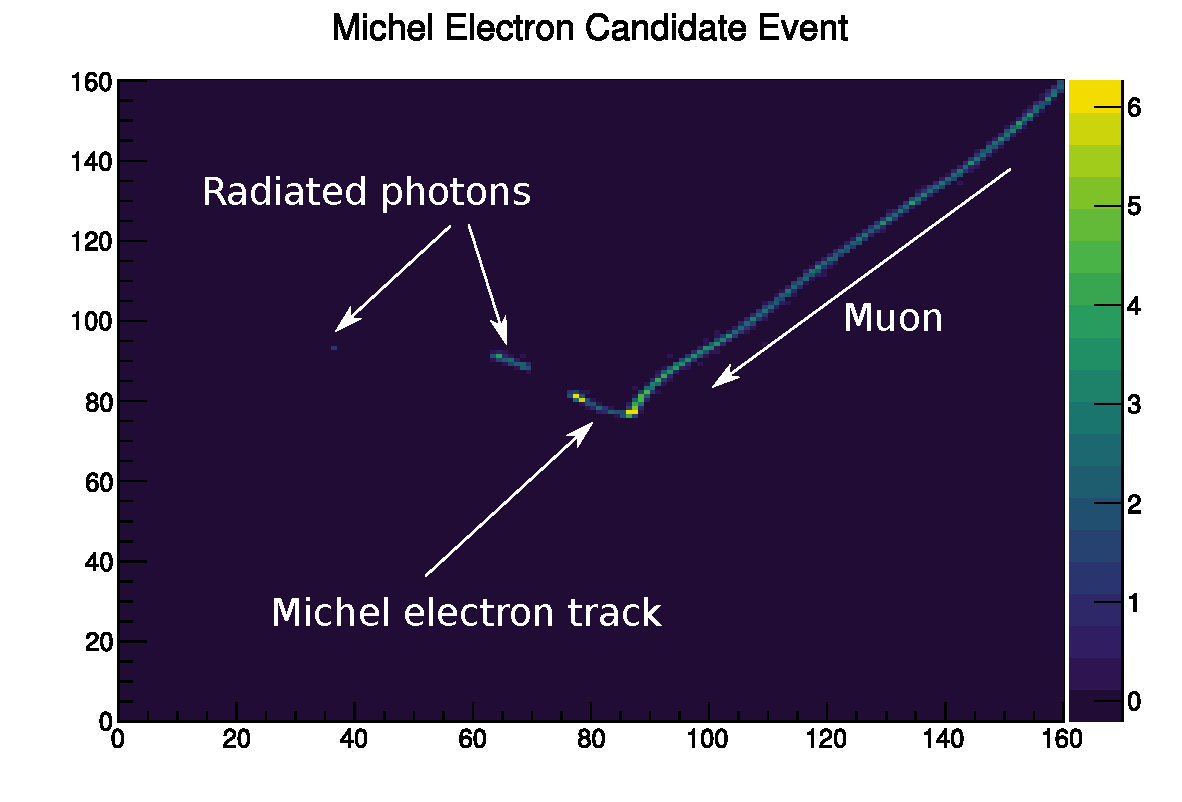
\includegraphics[width=0.7\textwidth]{figures/michel_candidate.pdf}
% 	\caption[Michel electron candidate event from ProtoDUNE--SP data.]{Michel 
% 	electron candidate event from ProtoDUNE--SP data.}
% 	\label{fig:michel_event}
% \end{figure}
%
%%%%%%%%%%%%%%%%%%%%%%%%%%%%%%%%%%%%%%%%%%%%%%%%%%%%%%%%%%%%%%%%%%%%%%%%%%%%%%%%

Studying electrons in the tens of MeV energy range can provide valuable input 
into reconstruction techniques and energy uncertainty for the measurement of
astrophysical neutrinos from supernova bursts. Understanding the response of
LArTPC detectors to electrons in this range will be important for any large
scale LArTPC experiment wishing to study supernova bursts. At these energies
electron interactions have large contributions from both ionisation energy loss
and radiative energy loss and therefore they have a unique signature which is 
neither track--like or shower--like. Low--energy electrons therefore require 
unique reconstruction algorithms to maximise the overall reconstruction 
performance. This chapter will discuss an approach to low--energy electron
reconstruction in LArTPC detectors based on the use of convolutional neural
networks and semantic segmentation. Michel electron events from \protodune{} will
be used to test the performance of this technique and to provide an estimate of
the energy uncertainty of LArTPC detectors for low--energy electrons.

\mccorrect{Chapter outline.}

\section{Michel Electrons in Liquid Argon} \label{ME_LAr}
\begin{mccorrection}
	Michel electrons
	\begin{itemize}
	\item Two types: at rest and captured
	\item Energy spectra
	\end{itemize}
\end{mccorrection}

Michel electrons are produced when a muon decays at rest. This decay gives rise
to a characteristic energy spectrum which has a sharp cut--off at around 50 MeV,
corresponding to half the muon mass. In matter it is also possible for $\mu^-$ 
to be captured on nuclei before they decay, this causes a broadening of the 
Michel electron spectrum for these events. A comparison of the Michel electron 
energy spectrum for free $\mu^+$ and captured $\mu^-$ is given in Fig.
\ref{fig:michel_spec}. The capture process occurs roughly 70\% of the time for
negative muons in liquid argon and therefore in \protodune{} the observed energy
spectrum is a combination of the two processes in roughly equal quantities.

\begin{figure}

	\centering

	\includegraphics[width=\textwidth]{figures/michel_spectra.pdf}

	\caption
	[Michel electron energy spectra in Liquid Argon]
	{Michel electron energy spectra in liquid argon. (a) free muons. (b) muon 
	capture at rest.}

	\label{fig:michel_spec}

\end{figure}

\begin{mccorrection}
	Electron and photon energy loss 
	\begin{itemize}
	\item Ionisation to radiative transition
	\item Event signature
	\item Example event
	\item Photon radiation length
	\item Photon spectrum
	\item Photon multiplicity
	\item Fractional energy loss vs energy
	\end{itemize}
\end{mccorrection}

As discussed in chapter \ref{ch:4-energyloss}, the energy loss for electrons in
liquid argon passes from an ionisation dominated regime to a radiation dominated
regime in the tens of MeV region. The crossover point for this transition occurs
at around 45 MeV, very close to the peak of the Michel electron spectrum. This
leads to a unique signature for Michel electrons in liquid argon detectors, a
short ($\sim$ 5cm) track segment is surrounded by a number of small radiated 
energy deposits. Figure \ref{fig:michel_event} shows an example of a Michel 
electron candidate from \protodune{} data, along with labels of the key 
features.

\begin{figure}
	\centering
	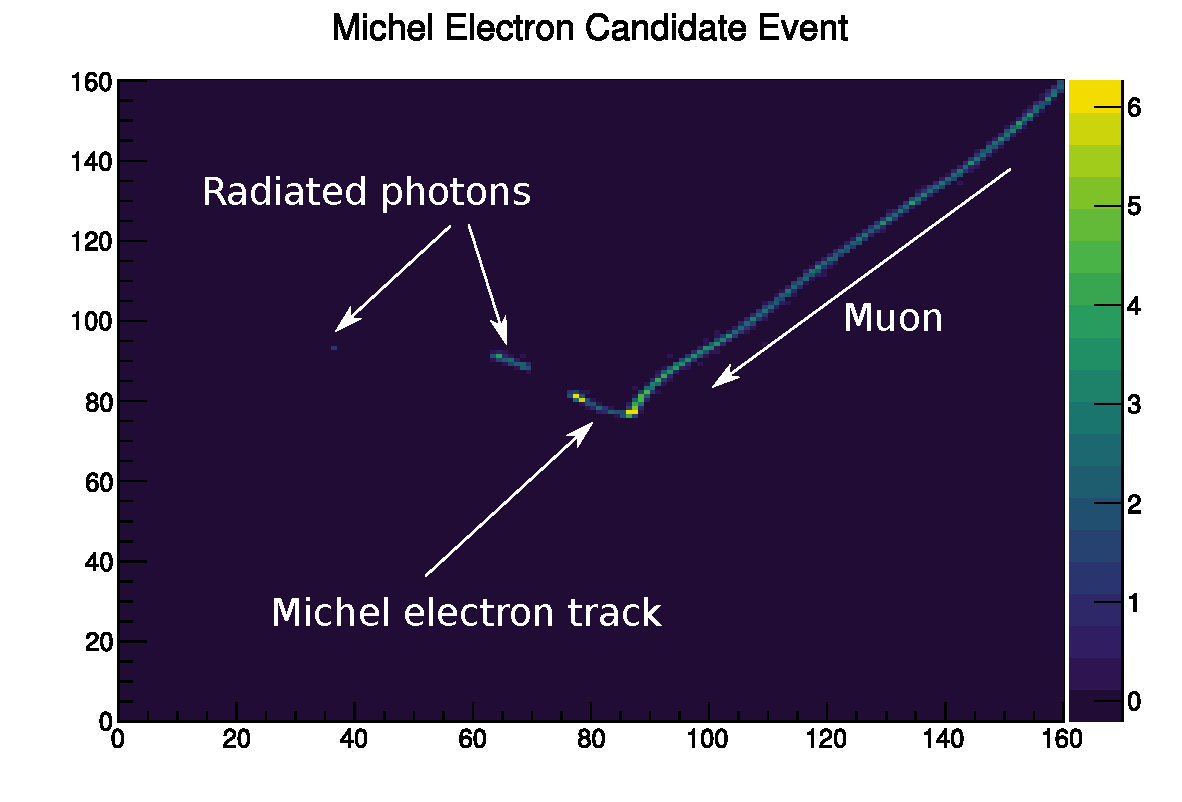
\includegraphics[width=\textwidth]{figures/michel_candidate.pdf}
	\caption
	[Michel electron candidate event from ProtoDUNE--SP data.]
	{Michel electron candidate event from ProtoDUNE--SP data.}
	\label{fig:michel_event}
\end{figure}

One of the main challenges for Michel electron reconstruction in liquid argon is
to successfully associate the radiated energy depositions back to the initial
Michel electron once they have produced ionisation in the detector. Photons have
a radiation length of around 20--30 cm in liquid argon which is many times
larger than the size of the typical track--like part of the event, around 5 cm. 
Fig. \ref{fig:photon_spec} shows the spectrum of radiated photons from Michel 
electron events in \protodune{} simulation alongside the photon multiplicity 
as a function of Michel electron energy. While most of the radiated photons 
only carry a small fraction of the Michel electrons energy, in some cases a 
single radiated photon can carry a significant fraction of the electron 
energy. In addition, around the peak of the Michel electron spectrum ($\sim$
45 MeV) there is a high photon multiplicity and a large spread in the
multiplicity distribution. The combination of these effects leads to a
significant spread in the fraction of radiated energy for Michel electron
events.

\begin{figure}
	% TODO: split into 2 figures
	\centering
	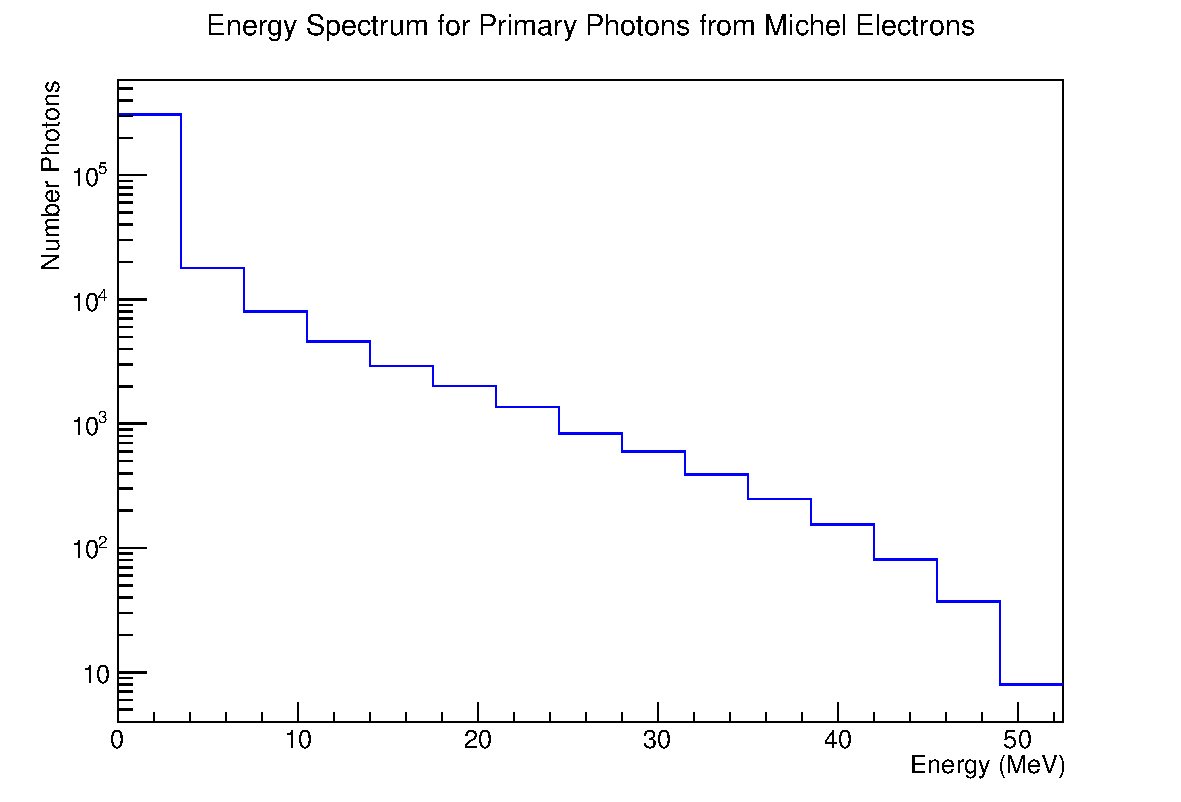
\includegraphics[width=\textwidth]{figures/photon_spec.pdf}
	\newline
	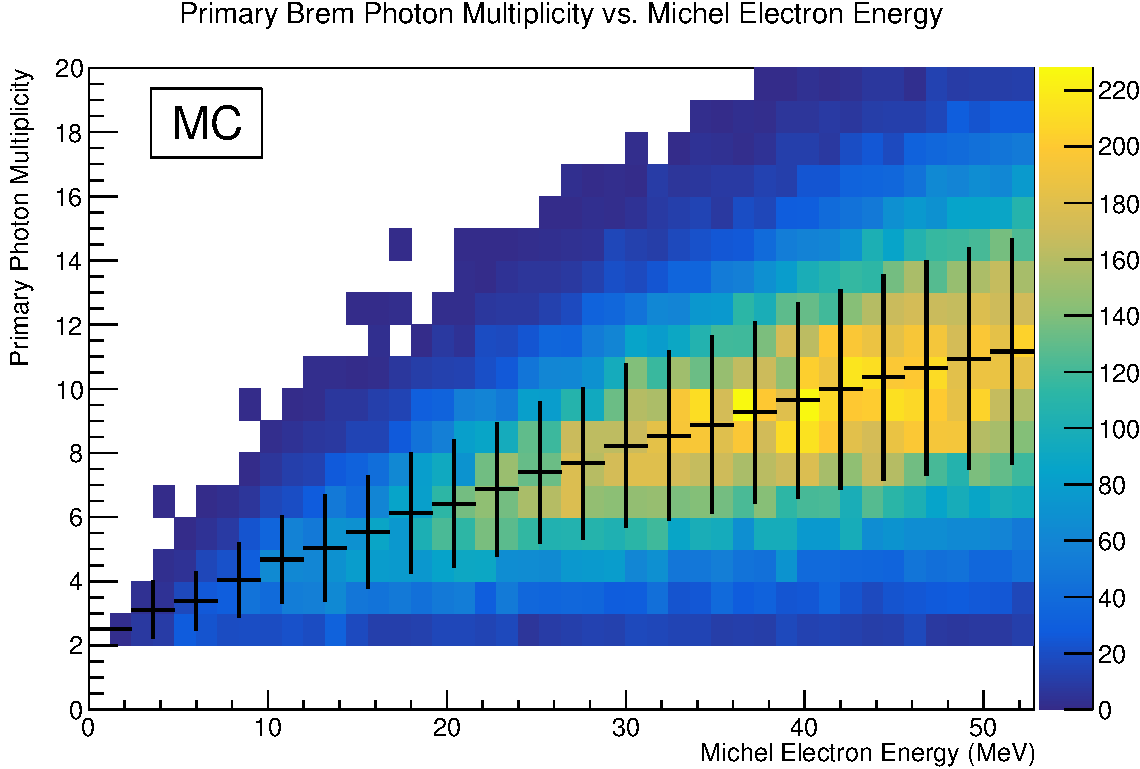
\includegraphics[width=\textwidth]{figures/photon_mult.pdf}
	\caption
	[Energy spectrum and multiplicity of radiated photons from Michel electron 
	events.]
	{Energy spectrum  and multiplicity of radiated photons from Michel electron events in
	\protodune{} simulation. 
	(a) Energy spectrum of radiated photons, log scale. 
	(b) Radiated photon multiplicity vs Michel electron energy. 
	}
	\label{fig:photon_spec}
\end{figure}

\mccorrect{Paragraph + figure on fraction of energy lost to radiation.}

\begin{mccorrection}
	Impact on event geometry and energy reco
	\begin{itemize}
	\item Track only ionisation
	\item Geometry of radiation
	\item 40cm ionisation 
	\item Need to collect radiative photons
	\end{itemize}
\end{mccorrection}

The energy which is lost into radiated photons is only visible once the photons
interact in the argon to produce secondary electrons which then ionise the
argon. These secondary electrons are scattered over large angles and distances
in the detector when compared to the short Michel electron track, the spatial 
distribution of secondary electrons is shown in Fig. \ref{fig:photon_geom}.
\mccorrect{TODO, analysis.}
\begin{figure}
	\centering
	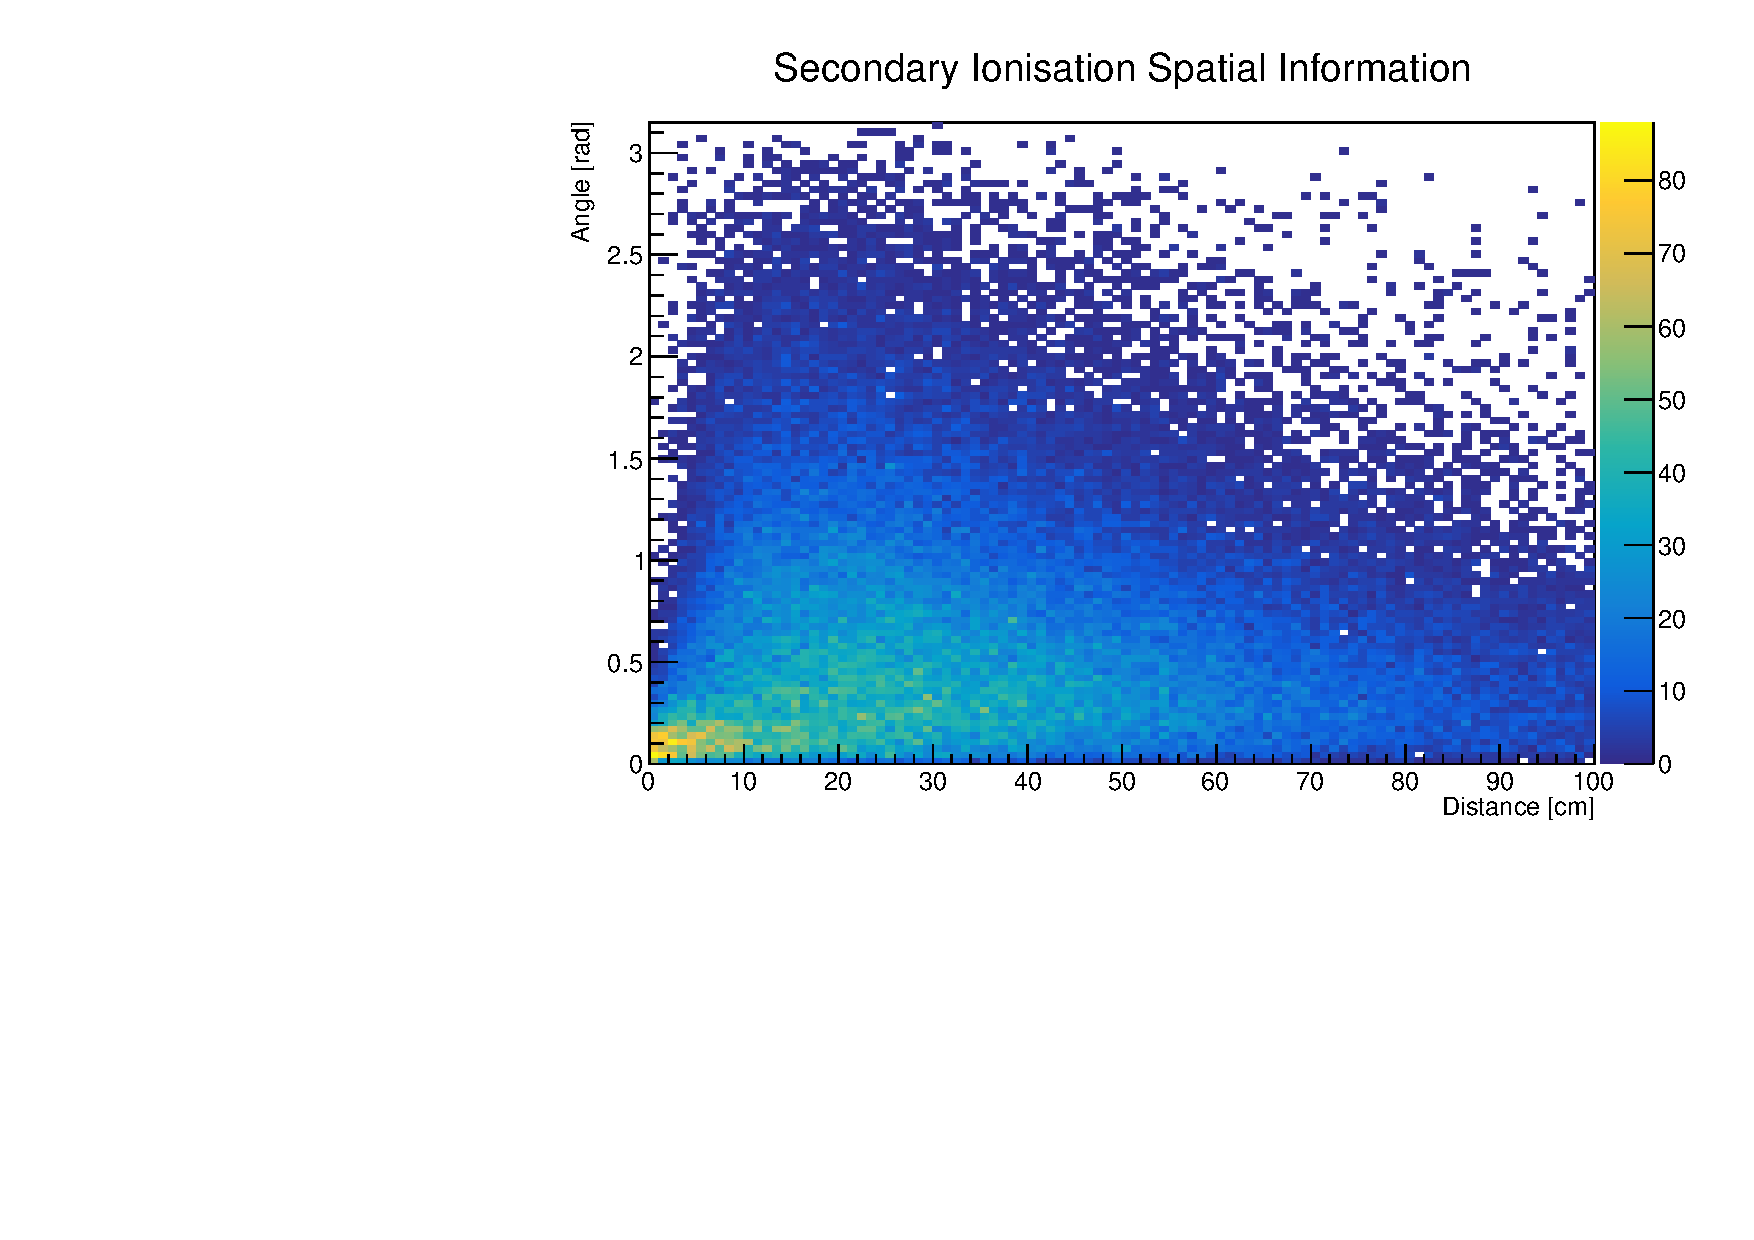
\includegraphics[width=\textwidth]{figures/photon_geom.pdf}
	\caption
	[Spatial distribution of radiated ionisation deposits.]
	{Spatial distribution of radiated ionisation deposits.}
	\label{fig:photon_geom}
\end{figure}

To highlight the impact of the radiated energy deposits we can consider the 
results of perfect energy reconstruction in two cases:
\begin{itemize}
	\item Only considering the Michel electron track.
	\item Considering all ionisation energy within some radius and angle of the 
		Michel electron track.
\end{itemize}
Fig. \ref{fig:michel_track_only} illustrates the considerable increase in energy
collected if radiated energy is considered, the distribution is significantly
narrower and much more energy is recovered when considering the energy deposited
within a cone of height 40cm and angle 30 \textdegree of the Michel electron
vertex. The average energy recovered is increased from \mccorrect{TODO \%} to
\mccorrect{TODO \%} and the spread is reduced from \mccorrect{TODO \%} to
\mccorrect{TODO \%}.
\begin{figure}
	\centering

	\begin{subfigure}{\textwidth}
		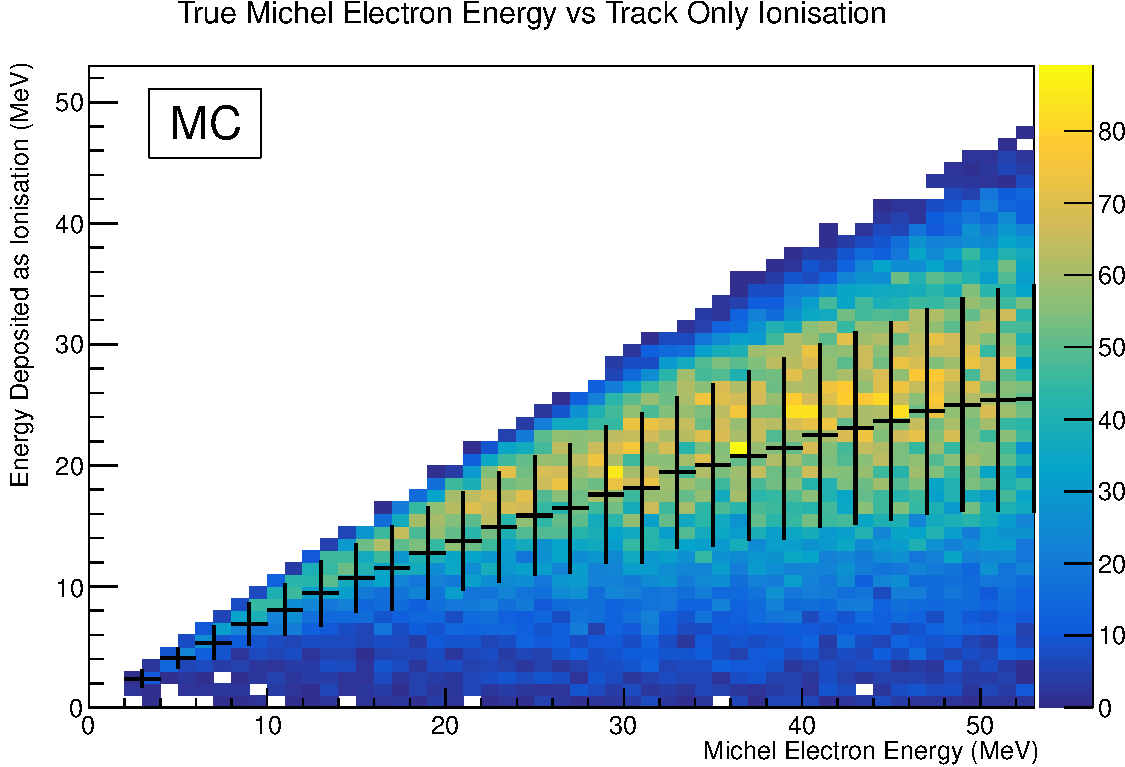
\includegraphics[clip, trim = 0cm 0cm 0cm 1cm, width=0.49\textwidth]{figures/michel_track_only.pdf}
		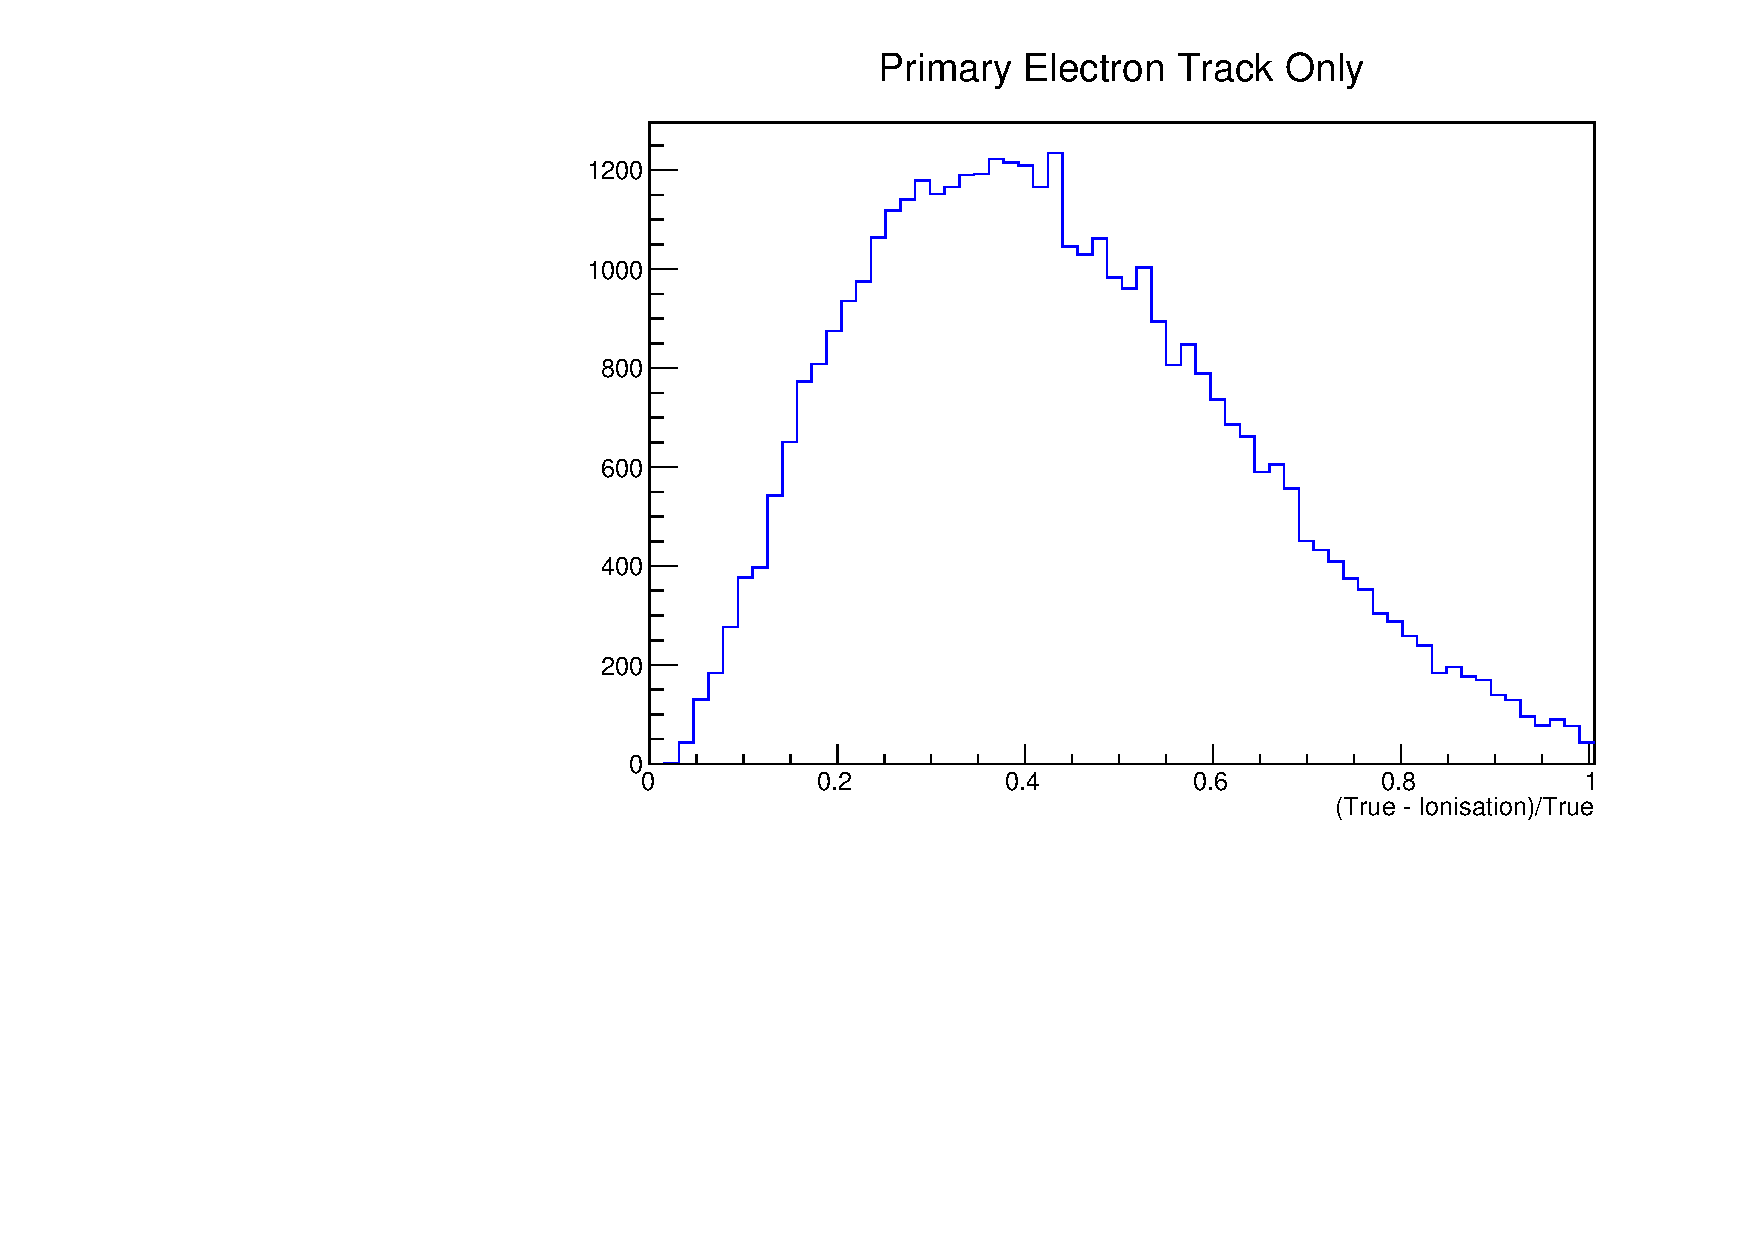
\includegraphics[clip, trim = 0cm 0cm 0cm 1cm, width=0.49\textwidth]{figures/track_frac.pdf}
	\end{subfigure}
	\begin{subfigure}{\textwidth}
		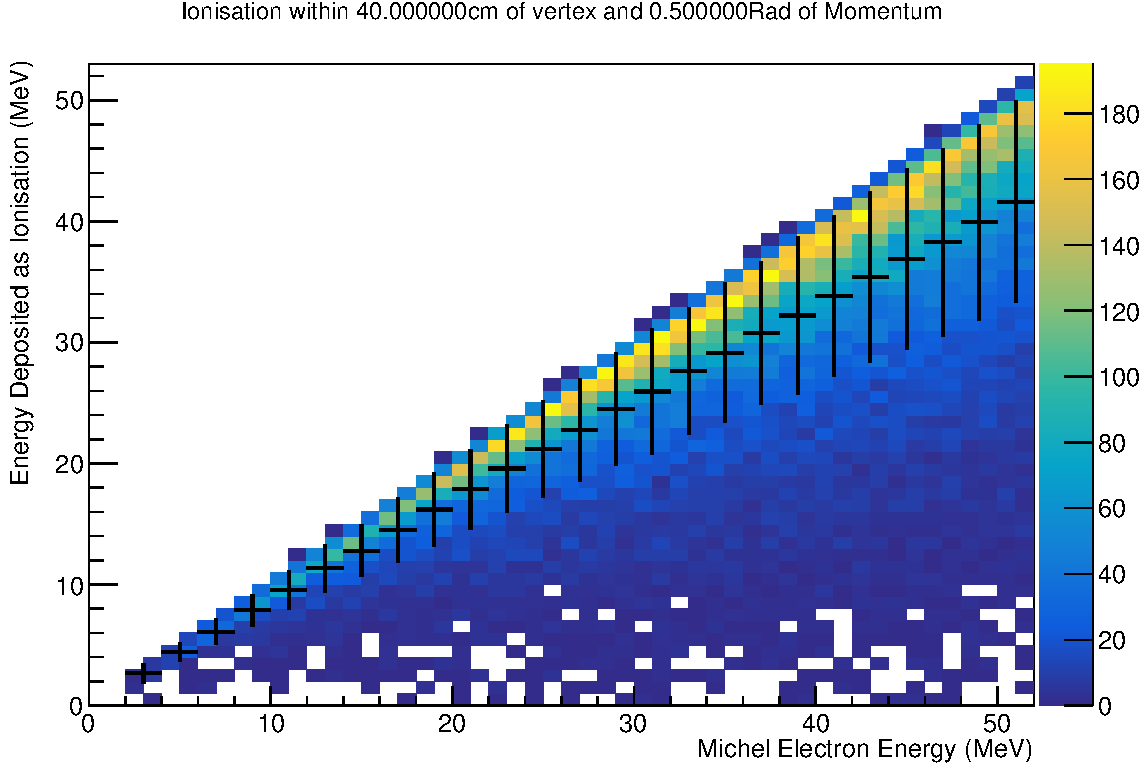
\includegraphics[clip, trim = 0cm 0cm 0cm 1cm, width=0.49\textwidth]{figures/cone_reco.pdf}
		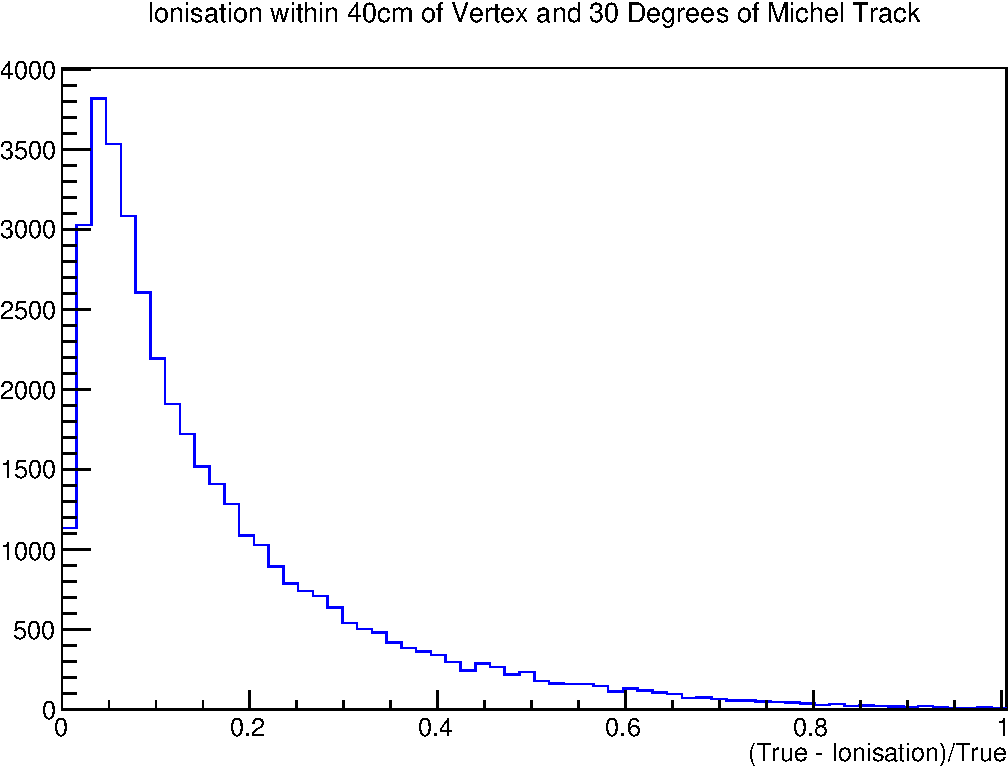
\includegraphics[clip, trim = 0cm 0cm 0cm 1cm, width=0.49\textwidth]{figures/cone_frac.pdf}
	\end{subfigure}

	\caption
	[Comparison of track--only ionisation and ionisation within a collection cone.]
	{Comparison of track--only ionisation and ionisation within a collection cone.}

	\label{fig:michel_track_only}

\end{figure}

\mccorrect{TODO, figure and paragraph for energy fraction vs radius.}
\begin{figure}
	\centering
	% TODO
	\includegraphics[width=\textwidth]{figures/frac_v_radius.pdf}
	\caption
	[Fraction of Michel electron energy collected vs collection radius.]
	{Fraction of Michel electron energy collected vs collection radius.}
	\label{fig:frac_v_radius}
\end{figure}

The MC study presented here highlights the importance of radiated energy
deposits in Michel electron and other low--energy electron events. Based on
these results it is clear that to minimise energy uncertainties for these events
it is important to maximise the amount of energy collected from radiated 
photons. The rest of this chapter will discuss an algorithm which was developed 
to tackle this problem, and it's application on Michel electron events in 
\protodune{} data.

\section{Michel Electron Event Selection} \label{ME_ES}
\begin{mccorrection}
	\begin{itemize}
	\item Michel hit tagging CNN
	\item Hit tagging + clustering explanation
	\item Algorithm performance: purity and efficiency
	\item CNN distributions
	\item Data v MC event selection distributions
	\end{itemize}
\end{mccorrection}

In order to select Michel electrons in \protodune{} data, an event selection
algorithm was developed based on combining the results from the hit tagging CNN 
from the previous chapter with clustering performed by the main \protodune{} 
reconstruction framework, Pandora. 

The event selection algorithm proceeds in the following steps:
\begin{enumerate}
	\item Start with all primary tracks from Pandora.
	\item Define a set of Michel electron candidates from the list of all
		daughters of the track.
	\item Find the best Michel electron candidate from the list of Michel electron
		candidates.
	\item Select events where the best Michel electron candidate passes the event
		selection cuts.
\end{enumerate}

In the first step the initial sample of muon candidates is defined. All tracks
from the Pandora reconstruction chain which have been labelled as primary tracks
are considered.

The second step defines a set of Michel electron candidates for each track in
the sample. A Michel electron candidate is any daughter of the primary Pandora
track which satisfies the following conditions:
\begin{itemize}
	\item Starts within 5 cm of the primary track endpoint.
	\item Contains a minimum of 5 hits on the collection plane.
\end{itemize}

In the third step the Michel electron candidates are analysed in order to define
the best Michel electron candidate for each track. The best Michel electron
candidate is the Michel electron candidate with the largest fraction of
Michel--like hits based on the output of the Michel electron score from the CNN
with a threshold of 0.9. In the case of a tie the Michel electron candidate with
the most hits is chosen.

The fourth step is the final decision, if the best Michel electron candidate is
made up of more than 80 \% of Michel--like hits then it is selected as a
Michel electron candidate.

Based on this algorithm Michel electron events are selected with over
\mccorrect{TODO \%} purity and \mccorrect{TODO \%} efficiency in \protodune{}
simulation. Figure \ref{fig:michel_like_frac} shows a comparison of the fraction of Michel--like
hits for the best Michel electron candidate in \protodune{} data and simulation.
\mccorrect{TODO, analysis and figure}.
\begin{figure}
	\centering
	% TODO
	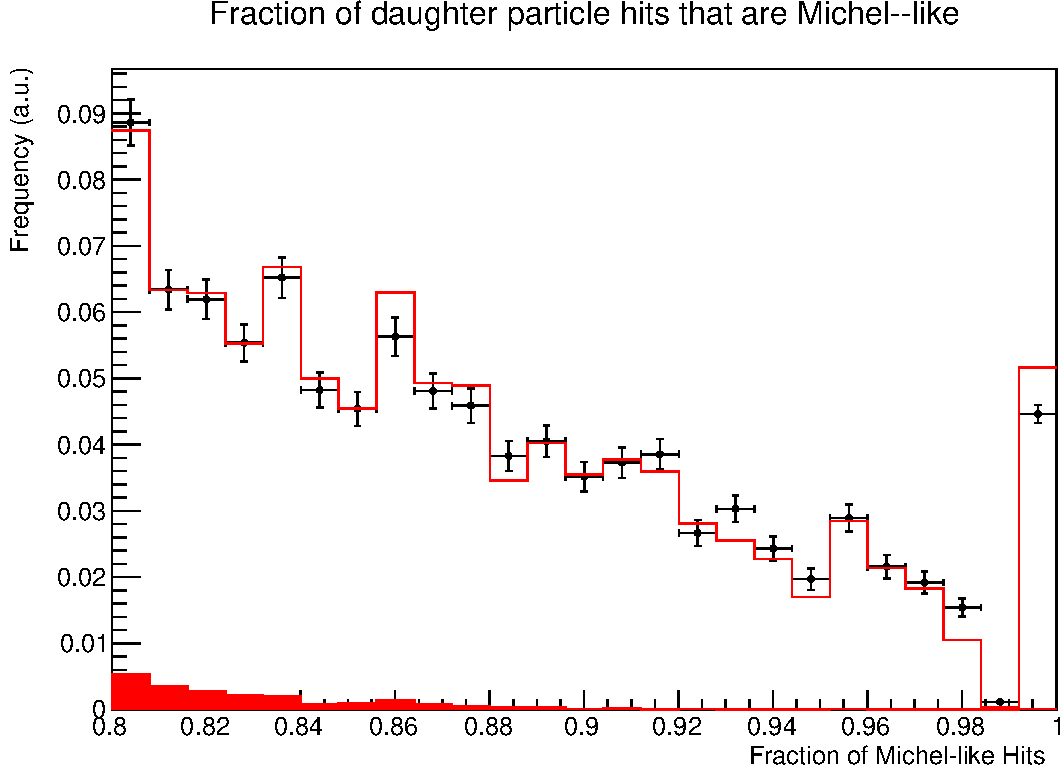
\includegraphics[width=\textwidth]{figures/michel_like_frac.pdf}
	\caption
	[Fraction of Michel--like hits in the best Michel electron candidate.]
	{Fraction of Michel--like hits in the best Michel electron candidate.}
	\label{fig:michel_like_frac}
\end{figure}

\mccorrect{TODO: Event selection distributions.}

\section{Michel Electron Energy Reconstruction} \label{ME_R} 
\begin{mccorrection}
	\begin{itemize} 
	\item U-Nets and semantic segmentation
	\item Algorithm outline
	\item Details of my U-Net
	\item Architecture plot
	\item Map examples
	\item Data v MC score distribution
	\item Reco spectrum
	\item NHits
	\item Energy per hit
	\item Reco geometry variables
	\end{itemize}
\end{mccorrection}

\section{Energy Uncertainty for Michel Electrons} \label{ME_EU}
\begin{mccorrection}
	\begin{itemize}
	\item Reco energy scaling
	\item Uncertainty vs energy
	\item Differences in dune far detector
	\end{itemize}
\end{mccorrection}

\chapter{\label{ch:7-implications}Implications for DUNE} 

\minitoc

This chapter will analyse the implications of the measured uncertainties on
analyses for the DUNE experiment. In particular the impact of the measured
energy scale uncertainty and energy scale bias on supernova neutrino physics in
DUNE will be analysed. The difference in conditions between ProtoDUNE--SP and
DUNE will be highlighted and the expected implications for energy scale
uncertainties in DUNE will be discussed.

The work for this section has yet to be started as it will be dependent on the
outcome of the Michel electron analysis in the previous section. I expect to be
able to start work on this analysis in September/October 2019 after preliminary
results of the Michel electron analysis; work for this section will be completed
by the end of December 2019.

\section{Supernova Neutrinos in DUNE}
\section{Impacts of Energy Uncertainties}

\chapter{\label{ch:8-conclusions}Conclusions} 

% \minitoc

This chapter will summarise the work presented in the thesis and provide
concluding remarks on the implications of the results for future analyses in
LArTPC experiments.



%% APPENDICES %% 
% Starts lettered appendices, adds a heading in table of contents, and adds a
% page that just says "Appendices" to signal the end of your main text.
% \startappendices
% Add or remove any appendices you'd like here:
% % \begin{savequote}[8cm]
% \textlatin{Cor animalium, fundamentum e\longs t vitæ, princeps omnium, Microco\longs mi Sol, a quo omnis vegetatio dependet, vigor omnis \& robur emanat.}
% 
% The heart of animals is the foundation of their life, the sovereign of everything within them, the sun of their microcosm, that upon which all growth depends, from which all power proceeds.
%   \qauthor{--- William Harvey \cite{harvey_exercitatio_1628}}
% \end{savequote}

\chapter{\label{app:1-example}Example Apendix}

\minitoc

\section{Example Apendix Title}

\label{sec:example}

Some example text.



%%%%% REFERENCES

\setlength{\baselineskip}{0pt} % JEM: Single-space References

{\renewcommand*\MakeUppercase[1]{#1}%
\printbibliography[heading=bibintoc,title={\bibtitle}]}

\end{document}
